% Options for packages loaded elsewhere
\PassOptionsToPackage{unicode}{hyperref}
\PassOptionsToPackage{hyphens}{url}
%
\documentclass[
  11pt,
  letterpaper,
  oneside,
  open=any]{scrbook}

\usepackage{amsmath,amssymb}
\usepackage{lmodern}
\usepackage{iftex}
\ifPDFTeX
  \usepackage[T1]{fontenc}
  \usepackage[utf8]{inputenc}
  \usepackage{textcomp} % provide euro and other symbols
\else % if luatex or xetex
  \usepackage{unicode-math}
  \defaultfontfeatures{Scale=MatchLowercase}
  \defaultfontfeatures[\rmfamily]{Ligatures=TeX,Scale=1}
  \setmainfont[]{Atkinson Hyperlegible}
  \setsansfont[]{Atkinson Hyperlegible}
\fi
% Use upquote if available, for straight quotes in verbatim environments
\IfFileExists{upquote.sty}{\usepackage{upquote}}{}
\IfFileExists{microtype.sty}{% use microtype if available
  \usepackage[]{microtype}
  \UseMicrotypeSet[protrusion]{basicmath} % disable protrusion for tt fonts
}{}
\makeatletter
\@ifundefined{KOMAClassName}{% if non-KOMA class
  \IfFileExists{parskip.sty}{%
    \usepackage{parskip}
  }{% else
    \setlength{\parindent}{0pt}
    \setlength{\parskip}{6pt plus 2pt minus 1pt}}
}{% if KOMA class
  \KOMAoptions{parskip=half}}
\makeatother
\usepackage{xcolor}
\usepackage[lmargin=1in,rmargin=1in,tmargin=1in,bmargin=1in]{geometry}
\setlength{\emergencystretch}{3em} % prevent overfull lines
\setcounter{secnumdepth}{-\maxdimen} % remove section numbering
% Make \paragraph and \subparagraph free-standing
\ifx\paragraph\undefined\else
  \let\oldparagraph\paragraph
  \renewcommand{\paragraph}[1]{\oldparagraph{#1}\mbox{}}
\fi
\ifx\subparagraph\undefined\else
  \let\oldsubparagraph\subparagraph
  \renewcommand{\subparagraph}[1]{\oldsubparagraph{#1}\mbox{}}
\fi

\usepackage{color}
\usepackage{fancyvrb}
\newcommand{\VerbBar}{|}
\newcommand{\VERB}{\Verb[commandchars=\\\{\}]}
\DefineVerbatimEnvironment{Highlighting}{Verbatim}{commandchars=\\\{\}}
% Add ',fontsize=\small' for more characters per line
\usepackage{framed}
\definecolor{shadecolor}{RGB}{241,243,245}
\newenvironment{Shaded}{\begin{snugshade}}{\end{snugshade}}
\newcommand{\AlertTok}[1]{\textcolor[rgb]{0.68,0.00,0.00}{#1}}
\newcommand{\AnnotationTok}[1]{\textcolor[rgb]{0.37,0.37,0.37}{#1}}
\newcommand{\AttributeTok}[1]{\textcolor[rgb]{0.40,0.45,0.13}{#1}}
\newcommand{\BaseNTok}[1]{\textcolor[rgb]{0.68,0.00,0.00}{#1}}
\newcommand{\BuiltInTok}[1]{\textcolor[rgb]{0.00,0.23,0.31}{#1}}
\newcommand{\CharTok}[1]{\textcolor[rgb]{0.13,0.47,0.30}{#1}}
\newcommand{\CommentTok}[1]{\textcolor[rgb]{0.37,0.37,0.37}{#1}}
\newcommand{\CommentVarTok}[1]{\textcolor[rgb]{0.37,0.37,0.37}{\textit{#1}}}
\newcommand{\ConstantTok}[1]{\textcolor[rgb]{0.56,0.35,0.01}{#1}}
\newcommand{\ControlFlowTok}[1]{\textcolor[rgb]{0.00,0.23,0.31}{#1}}
\newcommand{\DataTypeTok}[1]{\textcolor[rgb]{0.68,0.00,0.00}{#1}}
\newcommand{\DecValTok}[1]{\textcolor[rgb]{0.68,0.00,0.00}{#1}}
\newcommand{\DocumentationTok}[1]{\textcolor[rgb]{0.37,0.37,0.37}{\textit{#1}}}
\newcommand{\ErrorTok}[1]{\textcolor[rgb]{0.68,0.00,0.00}{#1}}
\newcommand{\ExtensionTok}[1]{\textcolor[rgb]{0.00,0.23,0.31}{#1}}
\newcommand{\FloatTok}[1]{\textcolor[rgb]{0.68,0.00,0.00}{#1}}
\newcommand{\FunctionTok}[1]{\textcolor[rgb]{0.28,0.35,0.67}{#1}}
\newcommand{\ImportTok}[1]{\textcolor[rgb]{0.00,0.46,0.62}{#1}}
\newcommand{\InformationTok}[1]{\textcolor[rgb]{0.37,0.37,0.37}{#1}}
\newcommand{\KeywordTok}[1]{\textcolor[rgb]{0.00,0.23,0.31}{#1}}
\newcommand{\NormalTok}[1]{\textcolor[rgb]{0.00,0.23,0.31}{#1}}
\newcommand{\OperatorTok}[1]{\textcolor[rgb]{0.37,0.37,0.37}{#1}}
\newcommand{\OtherTok}[1]{\textcolor[rgb]{0.00,0.23,0.31}{#1}}
\newcommand{\PreprocessorTok}[1]{\textcolor[rgb]{0.68,0.00,0.00}{#1}}
\newcommand{\RegionMarkerTok}[1]{\textcolor[rgb]{0.00,0.23,0.31}{#1}}
\newcommand{\SpecialCharTok}[1]{\textcolor[rgb]{0.37,0.37,0.37}{#1}}
\newcommand{\SpecialStringTok}[1]{\textcolor[rgb]{0.13,0.47,0.30}{#1}}
\newcommand{\StringTok}[1]{\textcolor[rgb]{0.13,0.47,0.30}{#1}}
\newcommand{\VariableTok}[1]{\textcolor[rgb]{0.07,0.07,0.07}{#1}}
\newcommand{\VerbatimStringTok}[1]{\textcolor[rgb]{0.13,0.47,0.30}{#1}}
\newcommand{\WarningTok}[1]{\textcolor[rgb]{0.37,0.37,0.37}{\textit{#1}}}

\providecommand{\tightlist}{%
  \setlength{\itemsep}{0pt}\setlength{\parskip}{0pt}}\usepackage{longtable,booktabs,array}
\usepackage{calc} % for calculating minipage widths
% Correct order of tables after \paragraph or \subparagraph
\usepackage{etoolbox}
\makeatletter
\patchcmd\longtable{\par}{\if@noskipsec\mbox{}\fi\par}{}{}
\makeatother
% Allow footnotes in longtable head/foot
\IfFileExists{footnotehyper.sty}{\usepackage{footnotehyper}}{\usepackage{footnote}}
\makesavenoteenv{longtable}
\usepackage{graphicx}
\makeatletter
\def\maxwidth{\ifdim\Gin@nat@width>\linewidth\linewidth\else\Gin@nat@width\fi}
\def\maxheight{\ifdim\Gin@nat@height>\textheight\textheight\else\Gin@nat@height\fi}
\makeatother
% Scale images if necessary, so that they will not overflow the page
% margins by default, and it is still possible to overwrite the defaults
% using explicit options in \includegraphics[width, height, ...]{}
\setkeys{Gin}{width=\maxwidth,height=\maxheight,keepaspectratio}
% Set default figure placement to htbp
\makeatletter
\def\fps@figure{htbp}
\makeatother
\newlength{\cslhangindent}
\setlength{\cslhangindent}{1.5em}
\newlength{\csllabelwidth}
\setlength{\csllabelwidth}{3em}
\newlength{\cslentryspacingunit} % times entry-spacing
\setlength{\cslentryspacingunit}{\parskip}
\newenvironment{CSLReferences}[2] % #1 hanging-ident, #2 entry spacing
 {% don't indent paragraphs
  \setlength{\parindent}{0pt}
  % turn on hanging indent if param 1 is 1
  \ifodd #1
  \let\oldpar\par
  \def\par{\hangindent=\cslhangindent\oldpar}
  \fi
  % set entry spacing
  \setlength{\parskip}{#2\cslentryspacingunit}
 }%
 {}
\usepackage{calc}
\newcommand{\CSLBlock}[1]{#1\hfill\break}
\newcommand{\CSLLeftMargin}[1]{\parbox[t]{\csllabelwidth}{#1}}
\newcommand{\CSLRightInline}[1]{\parbox[t]{\linewidth - \csllabelwidth}{#1}\break}
\newcommand{\CSLIndent}[1]{\hspace{\cslhangindent}#1}

\usepackage{booktabs}
\usepackage{longtable}
\usepackage{array}
\usepackage{multirow}
\usepackage{wrapfig}
\usepackage{float}
\usepackage{colortbl}
\usepackage{pdflscape}
\usepackage{tabu}
\usepackage{threeparttable}
\usepackage{threeparttablex}
\usepackage[normalem]{ulem}
\usepackage{makecell}
\usepackage{xcolor}
\makeatletter
\makeatother
\makeatletter
\@ifpackageloaded{bookmark}{}{\usepackage{bookmark}}
\makeatother
\makeatletter
\@ifpackageloaded{caption}{}{\usepackage{caption}}
\AtBeginDocument{%
\ifdefined\contentsname
  \renewcommand*\contentsname{Table of contents}
\else
  \newcommand\contentsname{Table of contents}
\fi
\ifdefined\listfigurename
  \renewcommand*\listfigurename{List of Figures}
\else
  \newcommand\listfigurename{List of Figures}
\fi
\ifdefined\listtablename
  \renewcommand*\listtablename{List of Tables}
\else
  \newcommand\listtablename{List of Tables}
\fi
\ifdefined\figurename
  \renewcommand*\figurename{Figure}
\else
  \newcommand\figurename{Figure}
\fi
\ifdefined\tablename
  \renewcommand*\tablename{Table}
\else
  \newcommand\tablename{Table}
\fi
}
\@ifpackageloaded{float}{}{\usepackage{float}}
\floatstyle{ruled}
\@ifundefined{c@chapter}{\newfloat{codelisting}{h}{lop}}{\newfloat{codelisting}{h}{lop}[chapter]}
\floatname{codelisting}{Listing}
\newcommand*\listoflistings{\listof{codelisting}{List of Listings}}
\makeatother
\makeatletter
\@ifpackageloaded{caption}{}{\usepackage{caption}}
\@ifpackageloaded{subcaption}{}{\usepackage{subcaption}}
\makeatother
\makeatletter
\@ifpackageloaded{tcolorbox}{}{\usepackage[many]{tcolorbox}}
\makeatother
\makeatletter
\@ifundefined{shadecolor}{\definecolor{shadecolor}{rgb}{.97, .97, .97}}
\makeatother
\makeatletter
\makeatother
\ifLuaTeX
  \usepackage{selnolig}  % disable illegal ligatures
\fi
\IfFileExists{bookmark.sty}{\usepackage{bookmark}}{\usepackage{hyperref}}
\IfFileExists{xurl.sty}{\usepackage{xurl}}{} % add URL line breaks if available
\urlstyle{same} % disable monospaced font for URLs
\hypersetup{
  pdftitle={Draft Proposal - Undergraduate Research Methods in Psychology},
  pdfauthor={Gordon Wright; Caroline Rix},
  hidelinks,
  pdfcreator={LaTeX via pandoc}}

\title{Draft Proposal - Undergraduate Research Methods in Psychology}
\usepackage{etoolbox}
\makeatletter
\providecommand{\subtitle}[1]{% add subtitle to \maketitle
  \apptocmd{\@title}{\par {\large #1 \par}}{}{}
}
\makeatother
\subtitle{BSc (Hons) Psychology and Streams, 2024/5 entry}
\author{Gordon Wright \and Caroline Rix}
\date{}

\begin{document}
\frontmatter
\maketitle
\ifdefined\Shaded\renewenvironment{Shaded}{\begin{tcolorbox}[interior hidden, boxrule=0pt, borderline west={3pt}{0pt}{shadecolor}, frame hidden, sharp corners, enhanced, breakable]}{\end{tcolorbox}}\fi

\renewcommand*\contentsname{Table of contents}
{
\setcounter{tocdepth}{2}
\tableofcontents
}
\mainmatter
\bookmarksetup{startatroot}

\hypertarget{proposal-for-ug-research-methods-2024-5}{%
\chapter{Proposal for UG Research Methods
2024-5}\label{proposal-for-ug-research-methods-2024-5}}

\raggedright

Goldsmiths as a college bullshit -

Goldsmiths as a department - differentiation, unique properties -
Interdisciplinary and methodologically rigorous and creative. Industry
links and all that jazz.

-\/-

We embrace an Open Science approach in our efforts to cultivate your
critical evaluation skills, enhance your understanding of the
significance - and power - of research, and equip you with the necessary
graduate-level skills to collect, handle, and interpret data using
programming software for statistical model development, visualisation
and analysis.

Through lectures, interactive group discussions, online skills
development modules, and practical lab sessions, we will ignite your
enthusiasm for Psychology and Behavioural Science research and help you
develop the fundamental skills, knowledge - and confidence - required to
become a Psychology literate, disruptive scientist of the future. Tada!

-\/-\/-

Communicate complex information effectively using appropriate written,
oral, graphical and electronic means, taking into account diversity
among individuals to whom the information is communicated.

Explain the potential impact of psychological research and theory on a
broad range of real world settings and situations (e.g., classrooms,
industry, commerce, healthcare, as well as local and global
communities).

Problem-solve and reason scientifically. Specifically, graduates will be
able to identify and pose research questions, consider alternative
approaches to their solutions, and evaluate outcomes.

Be sensitive to contextual and interpersonal factors. Graduates will be
familiar with the complexity of the factors that shape behaviour and
social interaction which, in turn, will make them more aware of the
bases of problems and interpersonal conflicts.

or Be a self-critical learner, showing sensitivity to contextual and
interpersonal factors. Graduates will be familiar with the complexity of
the factors that shape behaviour and social interaction which, in turn,
will make them more aware of the bases of problems and interpersonal
conflicts.

Show an understanding of various research paradigms, methods, and
evaluation procedures, including statistical analysis, as well as their
constraints.

Design, carry out, evaluate and interpret scientifically rigorous and
ethically sound studies both independently and collaboratively,
utilizing quantitative and qualitative methods, statistical analysis and
modern digital software.

Psychological literacy is the ability to understand and apply
psychological principles and theories to everyday life. This includes
the ability to understand how psychological processes and phenomena
influence our behavior, emotions, thoughts, and relationships. It also
includes the capacity to use psychological knowledge to make informed
decisions and to better understand, explain, and predict the behavior of
self and others.

Psychology graduates are highly sought after by employers due to their
ability to formulate and communicate well-reasoned, evidence-based, and
statistically defensible arguments based on their expertise in the study
of human behavior and its causes. On top of this, psychology graduates
possess the skills to work independently or collaboratively, as well as
strong numerical capabilities, verbal and written communication skills,
and an up-to-date knowledge of digital technologies applicable to a wide
range of occupational fields.

Intended Learning Outcomes

Create reproducible data analysis scripts and reports within the R
statistical programming environment.

QAA Benchmarks

Subject Knowledge and Understanding

6.3.4 demonstrate detailed knowledge of several specialised areas and/or
applications, some of which are at the cutting edge of research in the
discipline 6.3.5 demonstrate a systematic knowledge of a range of
research paradigms, research methods and measurement techniques,
including statistics and probability, and be aware of their limitations.

Subject-specific skills

PS510XX - RM1 - Introduction to Research Methods and Data Skills

PS520XX - RM2 - Research Methods in Practice and Data Skills

PS530XX - RM3 - Research Project Incubator

*PS710XX - Practical Research Skills

Lectures - Overview of key concepts/context and preview Lab practicals /
Data Skills

Labs - Practical or activity based (inc. Group Work)

\hypertarget{overview-of-rm-training}{%
\subsection{Overview of RM Training}\label{overview-of-rm-training}}

Y1 - showcase and active participation/skill development

Y2 - Practical drive towards self-motivated research

Y3 - Competent research

\hypertarget{pedagogical-overview}{%
\subsection{Pedagogical Overview}\label{pedagogical-overview}}

Social Constructivist

PeerMark

Podcast/Webpage/Blog

Integrate own interest/guided by stream/lab

\hypertarget{technical-overview}{%
\subsection{Technical Overview}\label{technical-overview}}

R will be used. Gold standard statistical programming language

For literate programming (The concept of
\href{https://en.wikipedia.org/wiki/Literate_programming}{\textbf{``literate
programming''}} was originally introduced by
\href{http://www.literateprogramming.com/knuthweb.pdf}{Donald Knuth} in
1984 )

Formerly RStudio. The Interactive Development Enviornment for use of R.

\hypertarget{hours-specification-years-1-2}{%
\subsection{Hours specification Years 1 \&
2}\label{hours-specification-years-1-2}}

\begin{longtable}[]{@{}lll@{}}
\caption{Notional Hours}\tabularnewline
\toprule()
Activity & Time & Note \\
\midrule()
\endfirsthead
\toprule()
Activity & Time & Note \\
\midrule()
\endhead
Lectures & 40 & 2hrs/week \\
Labs & 40 & 2hrs/week \\
Data Skills (Online) & 40 & 2hrs/week \\
Guided Reading/viewing & 40 & 2hrs/week \\
RPS & 20 & 1hr/week \\
Independent Study/Coursework & 120 & 6hr/week \\
\bottomrule()
\end{longtable}

\hypertarget{programme-overview}{%
\section{Programme Overview}\label{programme-overview}}

\hypertarget{pre-arrival-onwards-onboarding}{%
\subsection{Pre-Arrival onwards /
Onboarding}\label{pre-arrival-onwards-onboarding}}

Showcase in Induction week - Staff labs and research projects for the
year.

Year One students self-test

MSc Students - ditto and ability to shop around for supervision

Year 2 develop their pods? Show Y1 and Foundations what they did last
year

Year 3/MSc students - Research Bootcamp and refreshers/skills workshops

Support PhD students and staff

\hypertarget{shock-and-awe---shatter-the-a-level-preconceptions}{%
\subsection{Shock and Awe - Shatter the A-Level
preconceptions}\label{shock-and-awe---shatter-the-a-level-preconceptions}}

\hypertarget{vertically-integrated-projects-via-labs}{%
\subsection{Vertically Integrated Projects via
`Labs'}\label{vertically-integrated-projects-via-labs}}

\hypertarget{heartdata-week-recruitment-forward-prep}{%
\subsection{HeartData week (recruitment \& forward
prep)}\label{heartdata-week-recruitment-forward-prep}}

Potentially Reading Week Term 2? Or week before/after?

Allows all levels of students to blitz data and to showcase their work
for external stakeholders and to make a department-wide event.

\bookmarksetup{startatroot}

\hypertarget{stuff}{%
\chapter{STUFF}\label{stuff}}

\textbf{Personal development skills}

\begin{itemize}
\item
  self-management
\item
  team working
\item
  problem solving
\item
  application of information skills
\item
  communication
\item
  application of numeracy skills
\item
  specialist skills
\end{itemize}

\hypertarget{level-4---topline-summary}{%
\section{Level 4 - topline summary}\label{level-4---topline-summary}}

\hypertarget{module-content}{%
\subsection{Module Content}\label{module-content}}

This module equips students with the practical and conceptual skills
necessary for the effective study of psychology. It includes computer
skills, presenting results of experiments, structuring an essay, and
critiquing a scientific paper. Additionally, it provides an introduction
to experimental design, data, and statistics in psychology. Students
will learn the theoretical aspects of basic statistical concepts and
tests, and gain experience using statistical packages.

\hypertarget{module-learning-outcomes}{%
\subsection{Module Learning Outcomes}\label{module-learning-outcomes}}

The student should be able to:

demonstrate a comprehensive understanding of the principles of
experimental psychology, from reading and summarizing scientific papers
to planning, writing and presenting essays, reports and presentations.

understand the importance and relevance of data analysis, the different
types of experiments and tests used.

understand the philosophical underpinnings of qualitative and
quantitative approaches to research and evaluate their merits.

demonstrate the skills to analyse and interpret data using qualitative
and quantitative frameworks and methods.

demonstrate statistical proficiency in the ability to use R to compute
summary statistics, z-scores, chi-square, binomial tests, and parametric
and non-parametric comparison of two means.

be able to visualise and present/communicate research findings to a
range of audiences

select and provide a rationale for using a statistical test to analyse a
particular dataset, and present the results correctly in both graphical
and APA format.

\hypertarget{assessment}{%
\subsection{Assessment}\label{assessment}}

\begin{longtable}[]{@{}lllll@{}}
\toprule()
Assessment Element & Length & \% & F or S & LO Tested \\
\midrule()
\endhead
& & & & \\
& & & & \\
RPS & & & & \\
\bottomrule()
\end{longtable}

\hypertarget{reading-and-resource-list}{%
\subsection{Reading and Resource List}\label{reading-and-resource-list}}

We have a custom made textbook to support key study skills throughout
your degree:

\newpage

\begin{longtable}[]{@{}
  >{\centering\arraybackslash}p{(\columnwidth - 4\tabcolsep) * \real{0.0694}}
  >{\raggedright\arraybackslash}p{(\columnwidth - 4\tabcolsep) * \real{0.4306}}
  >{\raggedright\arraybackslash}p{(\columnwidth - 4\tabcolsep) * \real{0.3750}}@{}}
\caption{Y1 Term 1 Laydown}\tabularnewline
\toprule()
\begin{minipage}[b]{\linewidth}\centering
We ek
\end{minipage} & \begin{minipage}[b]{\linewidth}\raggedright
Lecture
\end{minipage} & \begin{minipage}[b]{\linewidth}\raggedright
Practical
\end{minipage} \\
\midrule()
\endfirsthead
\toprule()
\begin{minipage}[b]{\linewidth}\centering
We ek
\end{minipage} & \begin{minipage}[b]{\linewidth}\raggedright
Lecture
\end{minipage} & \begin{minipage}[b]{\linewidth}\raggedright
Practical
\end{minipage} \\
\midrule()
\endhead
P re & \begin{minipage}[t]{\linewidth}\raggedright
Preparing to become a Psychologist

\begin{verbatim}
<i class
\end{verbatim}

=``fa-solid fa-file-pdf''\textgreater{}
\end{minipage} & \\
WW & Let's measure some stuff & \\
1 & \textbf{Lecture:} Lorem Ipsem & \textbf{Reading:} Scarf adghsdbsG
gdsg as ash ah a ah rdhad fh ad. h j j j asd hasf ha dr hadfj \\
& \textbf{Lab:} Lorem Ipsem & \textbf{Data:} Snarg \\
2 & Finding patterns and relationships & \\
3 & Correlations and models & \\
4 & Distributions and sampling & \\
5 & Probabilities and P-Values & \\
RW & -\/- & -\/- \\
6 & Open Science, Reporting and Critique & \\
7 & Qualitative Research & \\
8 & Correlational Research & \\
9 & Q u asi-Experimental Research & \\
10 & Experimental Research & \\
\bottomrule()
\end{longtable}

\begin{longtable}[]{@{}
  >{\centering\arraybackslash}p{(\columnwidth - 4\tabcolsep) * \real{0.2361}}
  >{\centering\arraybackslash}p{(\columnwidth - 4\tabcolsep) * \real{0.2500}}
  >{\centering\arraybackslash}p{(\columnwidth - 4\tabcolsep) * \real{0.2639}}@{}}
\toprule()
\begin{minipage}[b]{\linewidth}\centering
Term 2
\end{minipage} & \begin{minipage}[b]{\linewidth}\centering
\end{minipage} & \begin{minipage}[b]{\linewidth}\centering
\end{minipage} \\
\midrule()
\endhead
1 & Statistical Models & Reproducibility \\
2 & Inferential Statistics & \\
3 & Alpha, Power, Effect and Sample Size & \\
4 & Correlation & \\
5 & Regression & \\
RW & -\/- & -\/- \\
6 & Multiple Regression & \\
7 & Logistic Regression & \\
8 & Comparing two means & \\
9 & Comparing several means & \\
10 & Data Skills for Employability & \\
\bottomrule()
\end{longtable}

Y1 Term 2 Laydown

\begin{longtable}[]{@{}
  >{\raggedright\arraybackslash}p{(\columnwidth - 8\tabcolsep) * \real{0.1389}}
  >{\raggedright\arraybackslash}p{(\columnwidth - 8\tabcolsep) * \real{0.1389}}
  >{\raggedright\arraybackslash}p{(\columnwidth - 8\tabcolsep) * \real{0.1389}}
  >{\raggedright\arraybackslash}p{(\columnwidth - 8\tabcolsep) * \real{0.1389}}
  >{\raggedright\arraybackslash}p{(\columnwidth - 8\tabcolsep) * \real{0.1389}}@{}}
\toprule()
\begin{minipage}[b]{\linewidth}\raggedright
Sem. 1: Week 1
\end{minipage} & \begin{minipage}[b]{\linewidth}\raggedright
R esearch Design \& Data
\end{minipage} & \begin{minipage}[b]{\linewidth}\raggedright
{[}Sli des{]} ( h ttp\%20s : \% 20//uoe \% 2 0psy.gi \% 2 0t\%20hu b .
io/dap\% 2 0 \%20r1/2 2 2 3\%20/le c \% 20tur\%2 0 e s/dapR1 \% 2
\%200\_le c 1 \_Res\%20 e a \%20rchD e \% 20sign- D \% 20a\%20t a .
html\#1)
\end{minipage} & \begin{minipage}[b]{\linewidth}\raggedright
\href{h\%2\%200\%20\%20\%20t\%\%2020\%20tp\%20s\%\%2020://uo\%20ep\%\%20\%\%202020\%20\%20\%20sy.g\%20\%20i\%20\%20th\%20ub\%20.\%20\%20\%20i\%20o\%2\%200/d\%2\%2\%2000\%20ap\%20r1/222\%\%2020\%20\%2\%20\%20\%200\%203/l\%20a\%20\%20bs/1\%20_\%20\%20\%20\%2001\%2\%200\%20_de\%20s\%20i\%2\%200\%20gn_\%20an\%20\%2\%200d\%20_\%\%2020\%20d\%\%2020a\%20t\%20a.html}{L
ab}
\end{minipage} & \begin{minipage}[b]{\linewidth}\raggedright
\href{ht\%20\%20t\%20\%20ps\%20:/\%20/\%20\%20\%20u\%20o\%2\%200ep\%2\%2\%2000\%20sy\%20.githu\%\%2020\%20\%2\%20\%20\%200\%20b.i\%20o\%20\%20/dap\%20r\%20\%20\%20\%201/\%2\%200\%20222\%203\%20/\%2\%200\%20lab\%20s/\%20\%2\%200r\%20d\%\%2020\%201\%\%2020_\%200\%201.html}{Read
ing}
\end{minipage} \\
\midrule()
\endhead
Sem. 1: Week 2 & D e s cribing C a t e gorical Data &
\protect\hyperlink{1}{S l ides} &
\href{ht\%2\%200\%20\%20\%20t\%\%2020\%20ps\%20:\%\%2020//uoe\%20ps\%\%20\%\%202020\%20\%20\%20y.gi\%20\%20t\%20\%20hu\%20b.\%20i\%20\%20\%20o\%20/\%2\%200da\%2\%2\%2000\%20pr\%201/2223\%\%2020\%20\%2\%20\%20\%200\%20/la\%20b\%20\%20s/1_\%200\%20\%20\%20\%202_\%2\%200\%20cat\%20e\%20g\%2\%200\%20ori\%20ca\%20\%2\%200l\%20_\%\%2020\%20d\%\%2020a\%20t\%20a.html}{L
a b} &
\href{ht\%20\%20t\%20\%20ps\%20:/\%20/\%20\%20\%20u\%20o\%2\%200ep\%2\%2\%2000\%20sy\%20.githu\%\%2020\%20\%2\%20\%20\%200\%20b.i\%20o\%20\%20/dap\%20r\%20\%20\%20\%201/\%2\%200\%20222\%203\%20/\%2\%200\%20lab\%20s/\%20\%2\%200r\%20d\%\%2020\%201\%\%2020_\%200\%202.html}{Read
ing} \\
Sem. 1: Week 3 & D e s cribing C o n tinuous Data & {[}Sl ides{]} (
htt\%20p \% 20s\%20: / /uo\%20\% 2 0epsy.g \% 20\%20i\% 2 0th\%20u b
.io/da\% \% 2020\%20 p r1/\%202 2 2\%203/l \% 20e\%20c t u\%2\%200 r
es/dapR \% 20\%2\%20 0 1\_l\%20e c 3\_De\%20 \% 20sc\%20 r ibi\%20n \%
20gCont \% 20D\%20a \% 20t\%20a . html\#1) & {[}Lab{]} ( h t tps://u \%
2 0 oepsy.g i t h u\%20b.i o / d apr1/\%2 0 2 2 23/labs / 1 \% 20\_03\_n
um e r ic\%20\_ d a t a.html) &
\href{ht\%20\%20t\%20\%20ps\%20:/\%20/\%20\%20\%20u\%20o\%2\%200ep\%2\%2\%2000\%20sy\%20.githu\%\%2020\%20\%2\%20\%20\%200\%20b.i\%20o\%20\%20/dap\%20r\%20\%20\%20\%201/\%2\%200\%20222\%203\%20/\%2\%200\%20lab\%20s/\%20\%2\%200r\%20d\%\%2020\%201\%\%2020_\%200\%203.html}{Read
ing} \\
Sem. 1: Week 4 & D e s cribing Re l a t i onships &
\begin{minipage}[t]{\linewidth}\raggedright
\hfill\break
{[} S lides{]} ( h t t ps://uo e p s y .github . i o / dapr1/2 2 2 3 /
lecture s / d a pR1\_lec 4 \_ D e scribin g R e l ationsh i p s .
html\#1)\strut
\end{minipage} & {[}Lab{]} ( h t t ps://uo e p s y .github . i o /
dapr1/2 22 3 / l abs/1\_ 0 4 \_ r elation s h i p s.html) &
\href{ht\%20\%20t\%20\%20ps\%20:/\%20/\%20\%20\%20u\%20o\%2\%200ep\%2\%2\%2000\%20sy\%20.githu\%\%2020\%20\%2\%20\%20\%200\%20b.i\%20o\%20\%20/dap\%20r\%20\%20\%20\%201/\%2\%200\%20222\%203\%20/\%2\%200\%20lab\%20s/\%20\%2\%200r\%20d\%\%2020\%201\%\%2020_\%200\%204.html}{Read
ing} \\
Sem. 1: Week 5 & F u nctions & \protect\hyperlink{1}{Slid e s} & {[}L
ab{]} (http\%2 0\%20\%20 s\%\%2020 :/\%20/\% 20uoeps y.\%\%20\% 2020\%20
\%20gith \%20u\%20 b.\%20io /\%20\%20 d\%20a\%2 0pr\%2\%2 00\%201/
2223/l\% 20\%20\%2 \%20\%200 abs\%20/ \%201\_05 \emph{\%20\%20 \%20fo\%2
0\%20rma t\%20i\%2 0\%20ve} re\%20\%2 0p\%20o\% 20\%20r\% 20t\%20\_
a.html) &
\href{ht\%20\%20t\%20\%20ps\%20:/\%20/\%20\%20\%20u\%20o\%2\%200ep\%2\%2\%2000\%20sy\%20.githu\%\%2020\%20\%2\%20\%20\%200\%20b.i\%20o\%20\%20/dap\%20r\%20\%20\%20\%201/\%2\%200\%20222\%203\%20/\%2\%200\%20lab\%20s/\%20\%2\%200r\%20d\%\%2020\%201\%\%2020_\%200\%205.html}{Read
ing} \\
Sem. 1: Week 6 & F o rmative f eedback week (A) & & & \\
Sem. 1: Week 7 & P r o b ability Theory & \protect\hyperlink{1}{Slid e
s} &
\href{h\%\%2020ttps:\%20//\%\%20\%\%202020\%20\%20\%20uoep\%20\%20s\%20\%20y.\%20gi\%20t\%20\%20\%20h\%20u\%2\%200b.\%2\%2\%2000\%20io\%20/dapr1\%\%2020\%20\%2\%20\%20\%200\%20/22\%202\%20\%203/la\%20b\%20\%20\%20\%20s/\%2\%200\%201_0\%207\%20_\%2\%200\%20pro\%20b_\%20\%2\%200t\%20h\%\%2020\%20e\%\%2020o\%20r\%20y.html}{La
b} &
\href{ht\%20\%20t\%20\%20ps\%20:/\%20/\%20\%20\%20u\%20o\%2\%200ep\%2\%2\%2000\%20sy\%20.githu\%\%2020\%20\%2\%20\%20\%200\%20b.i\%20o\%20\%20/dap\%20r\%20\%20\%20\%201/\%2\%200\%20222\%203\%20/\%2\%200\%20lab\%20s/\%20\%2\%200r\%20d\%\%2020\%201\%\%2020_\%200\%207.html}{Read
ing} \\
Sem. 1: Week 8 & P r o b ability Rules & \protect\hyperlink{1}{Slid e s}
& {[}L a b{]} ( h ttps:/\% 2 0 \%20/uoe p s y\%20.gi t \% 20hub\%2 0 .
io/dapr \% 2 \%2001/2 2 2 3/la\%20 b s \%20/1\_0 8 \% 20\_prob \_ \%
20r\%20u l e s.html) &
\href{ht\%20\%20t\%20\%20ps\%20:/\%20/\%20\%20\%20u\%20o\%2\%200ep\%2\%2\%2000\%20sy\%20.githu\%\%2020\%20\%2\%20\%20\%200\%20b.i\%20o\%20\%20/dap\%20r\%20\%20\%20\%201/\%2\%200\%20222\%203\%20/\%2\%200\%20lab\%20s/\%20\%2\%200r\%20d\%\%2020\%201\%\%2020_\%200\%208.html}{Read
ing} \\
Sem. 1: Week 9 & Random V a riables ( D i screte) &
\begin{minipage}[t]{\linewidth}\raggedright
\hfill\break
{[} S lides{]} ( h t t ps://uo e p s y .github . i o / dapr1/2 2 2 3 /
lecture s / d a pR1\_lec 8 \_ D i screteP r o b a bilityD i s t .
html\#1)\strut
\end{minipage} & {[}Lab{]} ( h t t ps://uo e p s y .github . i o /
dapr1/2 22 3 / l abs/1\_ 0 9 \_ d iscrete \_ d i s t.html) &
\href{ht\%20\%20t\%20\%20ps\%20:/\%20/\%20\%20\%20u\%20o\%2\%200ep\%2\%2\%2000\%20sy\%20.githu\%\%2020\%20\%2\%20\%20\%200\%20b.i\%20o\%20\%20/dap\%20r\%20\%20\%20\%201/\%2\%200\%20222\%203\%20/\%2\%200\%20lab\%20s/\%20\%2\%200r\%20d\%\%2020\%201\%\%2020_\%200\%209.html}{Read
ing} \\
Sem. 1: Week 10 & Random V a riables ( C o n t inuous) &
\protect\hyperlink{1}{S l ides} & {[}L ab{]} ( https:\% \% 2020\%20 /
/uo\%20e p s\%20y.g \% 20i\%20t h u\%2\%200 b .io/dap \% 20\%2\%20 0
r1/\%202 2 23/l\%20 \% 20ab\%20 s/ 1\_\%201 \% 200\_con \%2 0t\%20\_ \%
20d\%20i s t.html) &
\href{ht\%20\%20t\%20\%20ps\%20:/\%20/\%20\%20\%20u\%20o\%2\%200ep\%2\%2\%2000\%20sy\%20.githu\%\%2020\%20\%2\%20\%20\%200\%20b.i\%20o\%20\%20/dap\%20r\%20\%20\%20\%201/\%2\%200\%20222\%203\%20/\%2\%200\%20lab\%20s/\%20\%2\%200r\%20d\%\%2020\%201\%\%2020_\%201\%200.html}{Read
ing} \\
Sem. 1: Week 11 & S ampling & \protect\hyperlink{1}{Slide s} &
\href{htt\%20ps\%\%20\%\%202020\%20\%20\%20://u\%20\%20o\%20\%20ep\%20sy\%20.\%20\%20\%20g\%20i\%2\%200th\%2\%2\%2000\%20ub\%20.io/da\%\%2020\%20\%2\%20\%20\%200\%20pr1\%20/\%20\%202223\%20/\%20\%20\%20\%20la\%2\%200\%20bs/\%201\%20_\%2\%200\%2011_\%20sa\%20\%2\%200m\%20p\%\%2020\%20l\%\%2020i\%20n\%20g.html}{La
b} &
\href{ht\%20\%20t\%20\%20ps\%20:/\%20/\%20\%20\%20u\%20o\%2\%200ep\%2\%2\%2000\%20sy\%20.githu\%\%2020\%20\%2\%20\%20\%200\%20b.i\%20o\%20\%20/dap\%20r\%20\%20\%20\%201/\%2\%200\%20222\%203\%20/\%2\%200\%20lab\%20s/\%20\%2\%200r\%20d\%\%2020\%201\%\%2020_\%201\%201.html}{Read
ing} \\
\bottomrule()
\end{longtable}

\begin{longtable}[]{@{}
  >{\raggedright\arraybackslash}p{(\columnwidth - 8\tabcolsep) * \real{0.1667}}
  >{\raggedright\arraybackslash}p{(\columnwidth - 8\tabcolsep) * \real{0.1667}}
  >{\raggedright\arraybackslash}p{(\columnwidth - 8\tabcolsep) * \real{0.1667}}
  >{\raggedright\arraybackslash}p{(\columnwidth - 8\tabcolsep) * \real{0.1667}}
  >{\raggedright\arraybackslash}p{(\columnwidth - 8\tabcolsep) * \real{0.1667}}@{}}
\toprule()
\begin{minipage}[b]{\linewidth}\raggedright
Sem. 2: Week 1
\end{minipage} & \begin{minipage}[b]{\linewidth}\raggedright
C onfidence intervals
\end{minipage} & \begin{minipage}[b]{\linewidth}\raggedright
\href{http\%20s://\%20\%2\%200uoepsy.\%\%2020github\%\%2020.\%20io/\%20dapr1/2\%2\%20022\%203/l\%20ec\%20ture\%20s/da\%2\%20\%200pr1_2_01\%20_\%20conf\%\%2020int\%20_\%202223.pdf}{Sli
des}
\end{minipage} & \begin{minipage}[b]{\linewidth}\raggedright
{[}Lab{]} ( https://u o epsy.gith u b.io/dapr 1 /2223/lab s /2\_01\_con
f int.html)
\end{minipage} & \begin{minipage}[b]{\linewidth}\raggedright
\href{htt\%2\%200ps\%20://\%20uoeps\%2\%2\%2000y.githu\%20b.\%20i\%20\%20o/dapr\%20\%201/22\%2023\%20/\%20labs/\%20rd\%20\%202\%20_01.html}{Re
adi ng}
\end{minipage} \\
\midrule()
\endhead
Sem. 2: Week 2 & H ypothesis testing: p-values &
\href{ht\%20tps:\%20\%2\%200//uoeps\%\%2020y.gith\%\%2020u\%20b.i\%20o/dapr1\%2\%200/2\%20223\%20/l\%20ectu\%20res/\%2\%20\%200dapr1_2_\%200\%202_ht\%\%2020_pv\%20a\%20lues.pdf}{S
lid es} &
\href{ht\%20\%20tps:/\%\%2020/uoep\%2\%200sy\%20.gi\%20thub.\%2\%2\%2000io/dapr\%201/\%202\%20\%20223/la\%20\%20bs/2\%20_0\%202\%20_ht_p\%20va\%20\%20l\%20ues.html}{Lab}
&
\href{htt\%2\%200ps\%20://\%20uoeps\%2\%2\%2000y.githu\%20b.\%20i\%20\%20o/dapr\%20\%201/22\%2023\%20/\%20labs/\%20rd\%20\%202\%20_02.html}{Re
adi ng} \\
Sem. 2: Week 3 & H ypothesis testing: critical values & {[}Slid es{]} (
https://u \% 20oepsy.g i thub.\%20i o /dapr1/22 2 3\%20/lect u
res/dap\%2 0r 1\_2\_03\_h t \_cr\%20itv a lues.pdf) & {[}Lab{]}
(htt\%20ps \%20://uo\% 20epsy.\%2 0gi\%20thu b.io/\%2\%2 00dapr1/2
22\%203\%20 /labs/\%20 2\_03\%20\_h t\%20\_crit va\%20\%20l ues.html) &
\href{htt\%2\%200ps\%20://\%20uoeps\%2\%2\%2000y.githu\%20b.\%20i\%20\%20o/dapr\%20\%201/22\%2023\%20/\%20labs/\%20rd\%20\%202\%20_03.html}{Re
adi ng} \\
Sem. 2: Week 4 & C onnecting H ypothesis testing and c onfidence
intervals & {[}Slide s{]} (https:/\% 20/uoeps\% 20y\%20.gi thub.io\%2
0/d\%20apr 1/\%202223 /lec\%2\%20 0tures/da p\%20r1\_2\% 20\_04\%20\_
htci.pdf) &
\href{h\%\%2020ttps:\%2\%200//\%20uoe\%20psy.g\%2\%2\%2000ithub.i\%20o/\%20d\%20\%20apr1/2\%20\%20223/\%20la\%20b\%20s/2_0\%204_\%20\%20h\%20tci.html}{L
ab} &
\href{htt\%2\%200ps\%20://\%20uoeps\%2\%2\%2000y.githu\%20b.\%20i\%20\%20o/dapr\%20\%201/22\%2023\%20/\%20labs/\%20rd\%20\%202\%20_04.html}{Re
adi ng} \\
Sem. 2: Week 5 & Errors, Power, Effect size, and A s sumptions &
\href{htt\%20ps:/\%20\%2\%200/uoepsy\%\%2020.githu\%\%2020b\%20.io\%20/dapr1/\%2\%20022\%2023/\%20le\%20ctur\%20es/d\%2\%20\%200apr1_2_0\%205\%20_err\%\%2020ors\%20p\%20ower.pdf}{Sl
ide s} & {[}Lab{]} (htt\%20ps \%20://uo\% 20epsy.\%2 0gi\%20thu
b.io/\%2\%2 00dapr1/2 22\%203\%20 /labs/\%20 2\_05\%20\_h t\%20error
sp\%20\%20o wer.html) &
\href{htt\%2\%200ps\%20://\%20uoeps\%2\%2\%2000y.githu\%20b.\%20i\%20\%20o/dapr\%20\%201/22\%2023\%20/\%20labs/\%20rd\%20\%202\%20_05.html}{Re
adi ng} \\
\bottomrule()
\end{longtable}

\begin{longtable}[]{@{}
  >{\raggedright\arraybackslash}p{(\columnwidth - 4\tabcolsep) * \real{0.2361}}
  >{\raggedright\arraybackslash}p{(\columnwidth - 4\tabcolsep) * \real{0.3194}}
  >{\raggedright\arraybackslash}p{(\columnwidth - 4\tabcolsep) * \real{0.3194}}@{}}
\toprule()
\begin{minipage}[b]{\linewidth}\raggedright
0
\end{minipage} & \begin{minipage}[b]{\linewidth}\raggedright
\href{https:/\%2\%200/uo\%20epsy.\%20g\%20i\%20thub.io/\%20dap\%20r1/\%202122\%20/lect\%20ures\%\%2020/dapR\%201_\%20l\%20e\%20c0_CourseIntro.html}{Course
Intro}
\end{minipage} & \begin{minipage}[b]{\linewidth}\raggedright
\href{ht\%2\%200tps\%20://uo\%20e\%20p\%20sy.githu\%20b.i\%20o/d\%20apr1\%20/2122\%20/lab\%\%2020s/int\%20ro\%20_\%20r\%20_rstudio_year1.html}{Intro
to R \& RStu dio}
\end{minipage} \\
\midrule()
\endhead
1 &
\href{htt\%20\%20ps://\%20uoepsy.\%2\%200git\%20hub.i\%20o\%20/\%20dapr1/21\%2022/\%20lec\%20ture\%20s/dap\%20R1_l\%\%2020ec1_R\%20es\%20e\%20a\%20rchDesign-Data.html}{Research
Design \& Data} & {[}Data Typ es{]} ( http\%20s\%20://uoepsy .
gi\%20thub.io\%20/dapr 1 /21\%2022/la\%20bs\%20/ 1
\_01\_data\_types.html) \\
2 &
\href{https://u\%20\%20oepsy\%20.github\%2\%200.io\%20/dapr\%201\%20/\%202122/lec\%20tur\%20es/\%20dapR\%201_lec\%202_De\%\%2020scrib\%20in\%20g\%20C\%20ategoricalData.html}{Describing
Categorical Dat a} &
\href{https\%20:\%20/\%20/uoepsy.\%20git\%20hub\%20.io/\%20dapr1\%20/212\%\%20202/lab\%20s/\%201\%20_\%2002_categorical.html}{Categorical
Dat a} \\
3 &
\href{ht\%20\%20tps:/\%20/uoepsy\%2\%200.gi\%20thub.\%20i\%20o\%20/dapr1/2\%20122\%20/le\%20ctur\%20es/da\%20pR1_\%\%2020lec3_\%20De\%20s\%20c\%20ribingContData.html}{Describing
Continuous Data} &
\href{htt\%20p\%20s\%20://uoeps\%20y.g\%20ith\%20ub.i\%20o/dap\%20r1/2\%\%2020122/l\%20ab\%20s\%20/\%201_03_numerical.html}{Numerical
D ata} \\
4 &
\href{https:/\%20\%20/uoep\%20sy.gith\%2\%200ub.\%20io/da\%20p\%20r\%201/2122/l\%20ect\%20ure\%20s/da\%20pR1_l\%20ec4_\%\%2020Descr\%20ib\%20i\%20n\%20gRelationships.html}{Describing
Relationsh ips} & {[}Relationships{]} (h t t ps:/\%20/uoepsy.githu b. i
o /dapr1/2122/\%20labs/ 1\_ 0 4 \_relationships.html) \\
5 &
\href{https\%2\%200://\%20uoeps\%20y\%20.\%20github.i\%20o/d\%20apr\%201/21\%2022/le\%20ctur\%\%2020es/da\%20pR\%201\%20_\%20lec5_Functions.html}{F
unctions} &
\href{htt\%20p\%20s\%20://uoeps\%20y.g\%20ith\%20ub.i\%20o/dap\%20r1/2\%\%2020122/l\%20ab\%20s\%20/\%201_05_functions.html}{Functi
ons} \\
6 & -- Break Week -- & -- \\
7 &
\href{https\%20://uoep\%2\%200sy.\%20githu\%20b\%20.\%20io/dapr1\%20/21\%2022/\%20lect\%20ures/\%20dapR\%\%20201_lec\%206_\%20I\%20n\%20troProbability.html}{Intro
to Prob abilit y} &
\href{http\%2\%200s:/\%20/uoep\%20s\%20y\%20.github.\%20io/\%20dap\%20r1/2\%20122/l\%20abs/\%\%20201_07_\%20pr\%20o\%20b\%20ability_basics.html}{Probability
Basic s} \\
8 &
\href{https\%20://uoep\%2\%200sy.\%20githu\%20b\%20.\%20io/dapr1\%20/21\%2022/\%20lect\%20ures/\%20dapR\%\%20201_lec\%207_\%20P\%20r\%20obabilityRules.html}{Probability
Rule s} &
\href{htt\%2\%200ps:\%20//uoe\%20p\%20s\%20y.github\%20.io\%20/da\%20pr1/\%202122/\%20labs\%\%2020/1_08\%20_p\%20r\%20o\%20bability_rules.html}{Probability
Rul es} \\
9 &
\href{https:/\%20\%20/uoep\%20sy.gith\%2\%200ub.\%20io/da\%20p\%20r\%201/2122/l\%20ect\%20ure\%20s/da\%20pR1_l\%20ec8_\%\%2020Discr\%20et\%20e\%20P\%20robabilityDist.html}{Discrete
Probability Distributi ons} &
\href{h\%20ttps://\%2\%200uoe\%20psy.g\%20i\%20t\%20hub.io/d\%20apr\%201/2\%20122/\%20labs/\%201_09\%\%2020_disc\%20re\%20t\%20e\%20_distributions.html}{Discrete
Di stributio ns} \\
10 &
\href{https://u\%20\%20oepsy\%20.github\%2\%200.io\%20/dapr\%201\%20/\%202122/lec\%20tur\%20es/\%20dapR\%201_lec\%209_Co\%\%2020ntinu\%20ou\%20s\%20P\%20robabilityDist.html}{Continuous
Probability Distribution s} &
\href{htt\%20ps://uo\%2\%200eps\%20y.git\%20h\%20u\%20b.io/dap\%20r1/\%20212\%202/la\%20bs/1_\%2010_c\%\%2020ontin\%20uo\%20u\%20s\%20_distributions.html}{Continuous
Dist ributi ons} \\
11 &
\href{https\%20\%20://uo\%20epsy.gi\%2\%200thu\%20b.io/\%20d\%20a\%20pr1/2122\%20/le\%20ctu\%20res/\%20dapR1\%20_lec\%\%202010_Sa\%20mp\%20l\%20e\%20s-SamplingDist.html}{Samples
and Sampling Distributio ns} &
\href{h\%20ttps://\%2\%200uoe\%20psy.g\%20i\%20t\%20hub.io/d\%20apr\%201/2\%20122/\%20labs/\%201_11\%\%2020_samp\%20li\%20n\%20g\%20_distributions.html}{Sampling
Di stributio ns} \\
\bottomrule()
\end{longtable}

\hypertarget{semester-2}{%
\subsubsection{\texorpdfstring{\textbf{Semester
2}}{Semester 2}}\label{semester-2}}

\begin{longtable}[]{@{}
  >{\raggedright\arraybackslash}p{(\columnwidth - 4\tabcolsep) * \real{0.2361}}
  >{\raggedright\arraybackslash}p{(\columnwidth - 4\tabcolsep) * \real{0.3333}}
  >{\raggedright\arraybackslash}p{(\columnwidth - 4\tabcolsep) * \real{0.3056}}@{}}
\toprule()
\begin{minipage}[b]{\linewidth}\raggedright
\textbf{Week}
\end{minipage} & \begin{minipage}[b]{\linewidth}\raggedright
\textbf{Lecture}
\end{minipage} & \begin{minipage}[b]{\linewidth}\raggedright
\textbf{Workbook}
\end{minipage} \\
\midrule()
\endhead
1 &
\href{ht\%20tps\%20://uoepsy\%20\%20.githu\%20b.i\%20o/dapr1\%20/2122\%20/lectu\%20res\%20/d\%20a\%20pr1_2_01_confint.pdf}{Confidence
Interv als} &
\href{http\%20s:/\%20/uoep\%20sy.gi\%20thub.\%2\%200io/dapr1\%20/\%202122/la\%20bs/2_\%2001_c\%20onf\%20id\%20e\%20nce_intervals.html}{Confidence
Interval s} \\
2 &
\href{https\%20://\%20uoepsy.gi\%20\%20thub.i\%20o/d\%20apr1/21\%2022/le\%20ctures\%20/da\%20pr\%201\%20_2_02_ht_pvalues.pdf}{Hypothesis
Testing: P-Values} &
\href{ht\%20tps:/\%20/uoep\%2\%200sy.githu\%20b\%20.io/dap\%20r1/21\%2022/l\%20abs\%20/2\%20_\%2002_ht_pvalues.html}{Hypothesis
Testing: P-Value s} \\
3 &
\href{h\%20ttps://\%20uoe\%20psy.githu\%20\%20b.io/d\%20apr\%201/2122/\%20lectu\%20res/da\%20pr1\%20_2\%20_\%2003_ht_critvalues.pdf}{Hypothesis
Testing: Critical V alu es} &
\href{https\%20://uo\%20epsy.\%2\%200github.i\%20o\%20/dapr1/\%202122/\%20labs\%20/2_\%2003\%20_\%20ht_critvalues.html}{Hypothesis
Testing: Critical Va lues} \\
4 & {[}Hypothesis Testing \& Confidence Intervals{]} (h t
tps://uoe\%20psy.githu b. i o/dapr1/2122/le\%20ctu res /
dapr1\_2\_04\_htci.pdf) &
\href{h\%20ttps:\%2\%200//uoepsy\%20.\%20github.\%20io/da\%20pr1/\%20212\%202/\%20l\%20abs/2_04_htci.html}{Hypothesis
Testing \& Confidence Interva ls} \\
5 & {[}Errors, Power, Effect Size \& Assu mptions{]} (
https:\%20//uoepsy.git \% 20hub.io/da\%20pr1/212 2
/lectures/\%20dap\%20r1 \_ 2\_05\_errorspower.pdf) &
\href{https\%20://uo\%20epsy.\%2\%200github.i\%20o\%20/dapr1/\%202122/\%20labs\%20/2_\%2005\%20_\%20hterrorspower.html}{Errors,
Power, Effect Size \& Ass umpt ions} \\
6 & -- Break Week -- & -- \\
7 & {[}One Sample T-test{]} ( https:\%20//uoepsy.git \%
20hub.io/da\%20pr1/212 2 /lectures/\%20dap\%20r1 \_
lec16\_onesamplet.pdf) &
\href{ht\%20tps:/\%20/uoep\%2\%200sy.githu\%20b\%20.io/dap\%20r1/21\%2022/l\%20abs\%20/2\%20_\%2007_onesamplet.html}{One
Sample T-tes t} \\
8 &
\href{h\%20ttps://\%20uoe\%20psy.githu\%20\%20b.io/d\%20apr\%201/2122/\%20lectu\%20res/da\%20pr1\%20_l\%20e\%20c17_independentt.pdf}{Independent
Samples T -te st} & {[}Independent T-test{]} ( http\%20s://uoepsy\%2 0
.github.i\%20o/dapr1 / 2122/lab\%20s/2\%20\_0 8 \_independentt.html) \\
9 &
\href{htt\%20ps:\%20//uoepsy.\%20\%20github\%20.io\%20/dapr1/\%202122/\%20lectur\%20es/\%20da\%20p\%20r1_lec18_pairedt.pdf}{Paired
Samples T-te st} & {[}Paired T-test{]} (h t tps://u\%20oepsy.git hu b
.io/dapr1/212\%202/l ab s /2\_09\_pairedt.html) \\
10 &
\href{https\%20://\%20uoepsy.gi\%20\%20thub.i\%20o/d\%20apr1/21\%2022/le\%20ctures\%20/da\%20pr\%201\%20_lec19_Chisquare.pdf}{Chi-Square
Tests} &
\href{h\%20ttps:\%20//uoe\%2\%200psy.gith\%20u\%20b.io/da\%20pr1/2\%20122/\%20lab\%20s/\%202\%20_10_chisquare.html}{Chi-Square
Tes ts} \\
11 &
\href{h\%20ttps://\%20uoe\%20psy.githu\%20\%20b.io/d\%20apr\%201/2122/\%20lectu\%20res/da\%20pr1\%20_l\%20e\%20c20_Correlations.pdf}{Correla
tio ns} &
\href{htt\%2\%200ps://uoe\%20p\%20sy.gith\%20ub.io\%20/dap\%20r1/\%2021\%202\%202/2_11_covcor.html}{Covariance
\& Correl ation} \\
\bottomrule()
\end{longtable}

\newpage

\hypertarget{level-5---topline-summary}{%
\section{Level 5 - topline summary}\label{level-5---topline-summary}}

\hypertarget{module-aims}{%
\subsection{Module aims}\label{module-aims}}

Experimental designs in psychology typically employ statistical analyses
such as analysis of variance, factor analysis and regression. The aim of
this module is to make these topics more accessible through the use of
practical examples and data collection on a self-directed group research
project.

\hypertarget{module-content-1}{%
\subsection{Module Content}\label{module-content-1}}

The module's overall aim is to offer a supportive and intellectually
rigorous environment allowing students to develop highly valuable,
transferrable research and collaboration skills in the context of
undertaking a group research project.

This module teaches fundamental empirical research techniques within the
framework of Open Science and reproducibility, promoting best practice
in study design, Open Materials and Data, and methodological practice.
This module fully immerses students in the Goldsmiths `community of
practice,' providing structured research support and opportunities to
reflect on learning, modelling the key milestones of the final year
dissertation.

The module seeks to promote the application of a scientific,
intellectually virtuous, research-based approach to any and all future
endeavours, and integrates metacognitive and reflective practices to
deliver this transformative learning towards academic and personal
development.

Over the course of two terms students will follow a programme of
lectures introducing a critical approach to psychological research, as
well as how such skills can be transferred beyond psychology; across
academic disciplines and into the everyday world, with extensive use of
case studies and problem-based learning.

Structured weekly labs will enable students to work collaboratively to
identify an area of research, critically evaluate current research in
the area, and develop a modest research project building on these
insights.

Students will work together, alongside lab tutors and researchers in the
department, to design and deliver the research project, including
obtaining ethical approval, data collection and analysis, then
interpreting and writing up the results, and sharing the materials and
data in line with Open Science best practices in the Psychological,
Behavioural and Data Sciences.

\hypertarget{module-learning-outcomes-1}{%
\subsection{Module Learning Outcomes}\label{module-learning-outcomes-1}}

\begin{enumerate}
\def\labelenumi{\arabic{enumi}.}
\item
  Show a critical understanding of research design and methodology
\item
  Design, conduct, analyse, interpret and disseminate a psychological
  research project
\item
  Understand the conceptual and historical issues concerned with
  psychology as a science and area of practical application
\item
  Demonstrate valuable time-management and collaborative
  project-management skills and proficiencies
\item
  Reflect on their own learning, skill development and metacognition,
  preparing them for the final year dissertation
\item
  be able to use R to analyse: regression, correlations, reliability and
  validity, effect sizes, one-way within and between subjects designs
  (and post-hocs), two-way within, between and mixed designs; and factor
  analysis
\item
  Be able to present reproducible, APA format literate-programmed
  research reports.
\end{enumerate}

\hypertarget{assessment-1}{%
\subsection{Assessment}\label{assessment-1}}

\begin{longtable}[]{@{}lllll@{}}
\toprule()
Assessment Element & Length & \% & F or S & LO Tested \\
\midrule()
\endhead
& & & & \\
& & & & \\
RPS & & & & \\
\bottomrule()
\end{longtable}

\hypertarget{reading-and-resource-list-1}{%
\subsection{Reading and Resource
List}\label{reading-and-resource-list-1}}

We have a custom made textbook to support key study skills throughout
your degree:

\newpage

\hypertarget{semester-1}{%
\subsubsection{\texorpdfstring{\textbf{Semester
1}}{Semester 1}}\label{semester-1}}

\begin{longtable}[]{@{}
  >{\raggedright\arraybackslash}p{(\columnwidth - 4\tabcolsep) * \real{0.2361}}
  >{\raggedright\arraybackslash}p{(\columnwidth - 4\tabcolsep) * \real{0.3056}}
  >{\raggedright\arraybackslash}p{(\columnwidth - 4\tabcolsep) * \real{0.3056}}@{}}
\toprule()
\begin{minipage}[b]{\linewidth}\raggedright
\textbf{Week}
\end{minipage} & \begin{minipage}[b]{\linewidth}\raggedright
\textbf{Lecture}
\end{minipage} & \begin{minipage}[b]{\linewidth}\raggedright
\textbf{Workbook}
\end{minipage} \\
\midrule()
\endhead
1 & \begin{minipage}[t]{\linewidth}\raggedright
{[}Preli minaries{]} ( h ttps\%20://uoepsy.g\% 2 0 ithub.io/\%20dapr2/2
1 2 2/lectur\%20es/\%20da p r 2\_01\_Prelims.html)\\
\href{https:\%20/\%20/uo\%20epsy.gi\%\%2020\%20thub.io\%20/d\%20apr2\%20/21\%2022/le\%20cture\%20\%20s/d\%20ap\%20r\%202\%20_02_functions.html}{Functions
\& M odels}\strut
\end{minipage} & {[}Functions \& Mod els{]} ( https:\%\%2020//uoeps y
.\%20github.\%20io/da p r2/2\%20122\%20/l\%20a b
s/1\_01\_models.html) \\
2 & \begin{minipage}[t]{\linewidth}\raggedright
{[}Linear Model Intro{]} ( h ttps\%20://uoepsy.g\% 2 0
ithub.io/\%20dapr2/2 1 2 2/lectur\%20es/\%20da p r
2\_03\_LMintro.html)\\
\href{http\%20s\%20://\%20uoepsy.\%\%2020\%20github.\%20io\%20/dap\%20r2/\%202122/\%20lectu\%20\%20res\%20/d\%20a\%20p\%20r2_04_LMcoefs.html}{Linear
Model Coe ff icients}\strut
\end{minipage} &
\href{htt\%\%2020\%20ps://uo\%20ep\%20sy.g\%20ith\%20ub.io\%20/dapr\%20\%202/2\%2012\%202\%20/\%20labs/1_02_slr.html}{Simple
Linear Regr essi on} \\
3 & \begin{minipage}[t]{\linewidth}\raggedright
{[}Model Evalua tion{]} ( htt\%20ps://u\%20oeps y .githu\%\%2020b.io/da
p r\%202/2122/\%20lectu re s/d\%20apr\%202\_\%200 5
\_LMmodeleval.html)\\
\href{ht\%\%2020tps:\%20//uoep\%20s\%20y.g\%20ithub.i\%\%2020\%20o/dapr2\%20/2\%20122/\%20lec\%20tures\%20/dapr\%20\%202_0\%206_\%20L\%20M\%20standardized.html}{Standardized
Coefficient s}\\
{[}Binary Pr edictors{]} ( h ttps\%20://uoepsy.g\% 2 0
ithub.io/\%20dapr2/2 1 2 2/lectur\%20es/\%20da p r
2\_07\_LMBinary.html)\strut
\end{minipage} &
\href{ht\%20t\%20ps:\%20//uoeps\%\%2020\%20y.githu\%20b.\%20io/d\%20apr\%202/212\%202/lab\%20\%20s/1\%20_0\%203\%20_\%20slr_model_fit.html}{Model
F it} \\
4 & \begin{minipage}[t]{\linewidth}\raggedright
{[}Multiple Predic tors{]} ( htt\%20ps://u\%20oeps y
.githu\%\%2020b.io/da p r\%202/2122/\%20lectu re s/d\%20apr\%202\_\%200
8 \_LM\_multiple.html)\\
\href{h\%\%2020ttps\%20://uoe\%20p\%20sy.\%20github.\%\%2020\%20io/dapr\%202/\%202122\%20/le\%20cture\%20s/dap\%20\%20r2_\%2009\%20_\%20L\%20M_categorical.html}{Categorical
Predictors with \textgreater2 Leve ls}\strut
\end{minipage} &
\href{htt\%\%2020\%20ps://uo\%20ep\%20sy.g\%20ith\%20ub.io\%20/dapr\%20\%202/2\%2012\%202\%20/\%20labs/1_04_mlr.html}{Multiple
Linear Regr essi on} \\
5 &
\href{http\%20s://uo\%20e\%20psy\%20.github\%\%2020\%20.io/dap\%20r2\%20/212\%202/l\%20ectur\%20es/da\%20\%20pr2\%20_1\%200\%20_\%20interactions1.html}{Interactions
(Continuous * Categoric al)} & {[}Interactions I{]} (
https:\%\%2020//uoeps y .\%20github.\%20io/da p r2/2\%20122\%20/l\%20a b
s/1\_05\_int\_nc.html) \\
6 & -- Break Week -- & -- \\
7 &
\href{http\%20s://uo\%20e\%20psy\%20.github\%\%2020\%20.io/dap\%20r2\%20/212\%202/l\%20ectur\%20es/da\%20\%20pr2\%20_1\%200\%20_\%20interactions2.html}{Interactions
(Continuous * Continuo us)} & {[}Interactions II{]} (
https:\%\%2020//uoeps y .\%20github.\%20io/da p r2/2\%20122\%20/l\%20a b
s/1\_07\_int\_nn.html) \\
8 &
\href{http\%20s://uo\%20e\%20psy\%20.github\%\%2020\%20.io/dap\%20r2\%20/212\%202/l\%20ectur\%20es/da\%20\%20pr2\%20_1\%201\%20_\%20interactions3.html}{Interactions
(Categorical * Categoric al)} & {[}Interactions III{]} (
https:\%\%2020//uoeps y .\%20github.\%20io/da p r2/2\%20122\%20/l\%20a b
s/1\_08\_int\_cc.html) \\
9 & \begin{minipage}[t]{\linewidth}\raggedright
{[}Assumpt ions{]} ( htt\%20ps://u\%20oeps y .githu\%\%2020b.io/da p
r\%202/2122/\%20lectu re s/d\%20apr\%202\_\%201 2 \_assumptions.html)\\
\href{http\%20s://uo\%20e\%20psy\%20.github\%\%2020\%20.io/dap\%20r2\%20/212\%202/l\%20ectur\%20es/da\%20\%20pr2\%20_1\%203\%20_\%20diagnostics1.html}{Diagnostics
I}\\
{[}Diagnostics II{]} ( htt\%20ps://u\%20oeps y .githu\%\%2020b.io/da p
r\%202/2122/\%20lectu re s/d\%20apr\%202\_\%201 3
\_diagnostics2.html)\strut
\end{minipage} &
\href{h\%20ttp\%20s://uoe\%\%2020\%20psy.git\%20hu\%20b.io\%20/da\%20pr2/2\%20122/l\%20\%20abs\%20/1\%20_\%200\%209_assumptions.html}{Assumptions
\& Diag nostics} \\
10 & \begin{minipage}[t]{\linewidth}\raggedright
\href{htt\%\%2020ps:/\%20/uoeps\%20y\%20.gi\%20thub.io\%\%2020\%20/dapr2/\%2021\%2022/l\%20ect\%20ures/\%20dapr2\%20\%20_14\%20_B\%20o\%20o\%20tstrapTheory.html}{Bootstrap
Theory}\\
\href{ht\%20tps://\%20u\%20oep\%20sy.gith\%\%2020\%20ub.io/d\%20ap\%20r2/2\%20122\%20/lect\%20ures/\%20\%20dap\%20r2\%20_\%201\%204_BootstrapLM.html}{Bootstrap
for Regre ssi on}\strut
\end{minipage} &
\href{ht\%20t\%20ps:\%20//uoeps\%\%2020\%20y.githu\%20b.\%20io/d\%20apr\%202/212\%202/lab\%20\%20s/1\%20_1\%200\%20_\%20bootstrap_reg.html}{Bootstrapping
Regressi on} \\
11 & -- No Lecture -- &
\href{h\%20ttps://\%\%2020\%20uoepsy.\%20gi\%20thub\%20.io\%20/dapr\%202/212\%20\%202/l\%20ab\%20s\%20/\%201_11_write_up.html}{Writing
U p} \\
\bottomrule()
\end{longtable}

\hypertarget{semester-2-1}{%
\subsubsection{\texorpdfstring{\textbf{Semester
2}}{Semester 2}}\label{semester-2-1}}

\begin{longtable}[]{@{}
  >{\raggedright\arraybackslash}p{(\columnwidth - 4\tabcolsep) * \real{0.2361}}
  >{\raggedright\arraybackslash}p{(\columnwidth - 4\tabcolsep) * \real{0.3056}}
  >{\raggedright\arraybackslash}p{(\columnwidth - 4\tabcolsep) * \real{0.3056}}@{}}
\toprule()
\begin{minipage}[b]{\linewidth}\raggedright
\textbf{Week}
\end{minipage} & \begin{minipage}[b]{\linewidth}\raggedright
\textbf{Lecture}
\end{minipage} & \begin{minipage}[b]{\linewidth}\raggedright
\textbf{Workbook}
\end{minipage} \\
\midrule()
\endhead
1 &
\href{htt\%\%2020ps:/\%20/uoeps\%20y\%20.gi\%20thub.io\%\%2020\%20/dapr2/\%2021\%2022/l\%20ect\%20ures/\%20dapr2\%20\%20_15\%20_m\%20o\%20d\%20el_comparison.html}{Model
Co mparison} & {[}Model Comparison{]} (h t t ps://uo\%20epsy.gith ub . i
o/dapr2/2122/\%20lab s/ 2 \_ 01\_model\_comp.html) \\
2 &
\href{htt\%20ps://\%\%2020uoep\%20sy.git\%20h\%20ub.\%20io/dapr\%\%2020\%202/2122/\%20le\%20ctur\%20es/\%20dapr2\%20_16_c\%20\%20odi\%20ng\%20c\%20a\%20tegoricaldata.html}{Coding
Categorical Predic tors} &
\href{htt\%20p\%20s:/\%20/uoepsy\%\%2020\%20.github\%20.i\%20o/da\%20pr2\%20/2122\%20/labs\%20\%20/2_\%2002\%20_\%20c\%20oding_factors.html}{Coding
Categorical Predictor s} \\
3 &
\href{https\%\%2020://u\%20oepsy.\%20g\%20ith\%20ub.io/d\%\%2020\%20apr2/21\%2022\%20/lec\%20tur\%20es/da\%20pr2_1\%20\%207_e\%20xp\%20e\%20r\%20imentaldesign.html}{Experimental
D esigns} &
\href{http\%20s://uo\%20e\%20psy\%20.github\%\%2020\%20.io/dap\%20r2\%20/212\%202/l\%20abs/2\%20_03_c\%20\%20ont\%20_d\%20e\%20s\%20ign_factanova.html}{Contrasts,
Study Design \& Factorial AN OVA} \\
4 &
\href{htt\%\%2020ps:/\%20/uoeps\%20y\%20.gi\%20thub.io\%\%2020\%20/dapr2/\%2021\%2022/l\%20ect\%20ures/\%20dapr2\%20\%20_18\%20_f\%20a\%20c\%20torialdesigns.html}{Factorial
Designs} &
\href{http\%20s\%20://\%20uoepsy.\%\%2020\%20github.\%20io\%20/dap\%20r2/\%202122/\%20labs/\%20\%202_0\%204_\%20f\%20a\%20ctorial_anova.html}{Two-Way
ANOVA} \\
5 &
\href{htt\%20ps://\%\%2020uoep\%20sy.git\%20h\%20ub.\%20io/dapr\%\%2020\%202/2122/\%20le\%20ctur\%20es/\%20dapr2\%20_19_r\%20\%20evi\%20si\%20t\%20i\%20ngassumptions.html}{Multiple
Comparison \& Assumpt ions} &
\href{h\%20ttps:/\%20/\%20uoe\%20psy.git\%\%2020\%20hub.io/\%20da\%20pr2/\%20212\%202/lab\%20s/2_0\%20\%205_m\%20ul\%20t\%20i\%20_comp_writeup.html}{Assumptions,
Multiple Comparisons, Corrections \& Writing u p} \\
6 & -- Break Week -- & -- \\
7 & \begin{minipage}[t]{\linewidth}\raggedright
\href{htt\%\%2020ps:/\%20/uoeps\%20y\%20.gi\%20thub.io\%\%2020\%20/dapr2/\%2021\%2022/l\%20ect\%20ures/\%20dapr2\%20\%20_20\%20_b\%20i\%20n\%20arylogistic1.html}{Binary
Logistic Regression I}\\
\href{ht\%\%2020tps:\%20//uoep\%20s\%20y.g\%20ithub.i\%\%2020\%20o/dapr2\%20/2\%20122/\%20lec\%20tures\%20/dapr\%20\%202_2\%200_\%20b\%20i\%20narylogistic2.html}{Binary
Logistic Regression I I}\strut
\end{minipage} & {[}Logistic Regress ion{]} ( https:\%\%2020//uoeps y
.\%20github.\%20io/da p r2/2\%20122\%20/l\%20a b
s/2\_07\_binary.html) \\
8 & \begin{minipage}[t]{\linewidth}\raggedright
\href{https:\%20/\%20/uo\%20epsy.gi\%\%2020\%20thub.io\%20/d\%20apr2\%20/21\%2022/le\%20cture\%20\%20s/d\%20ap\%20r\%202\%20_21_introglm.html}{Intro
to the Generalised Linear Model (GLM)}\\
\href{htt\%\%2020ps:/\%20/uoeps\%20y\%20.gi\%20thub.io\%\%2020\%20/dapr2/\%2021\%2022/l\%20ect\%20ures/\%20dapr2\%20\%20_20\%20_i\%20n\%20t\%20romissingdata.html}{Intro
to Missing Data}\strut
\end{minipage} &
\href{h\%20t\%20tps\%20://uoep\%\%2020\%20sy.gith\%20ub\%20.io/\%20dap\%20r2/21\%2022/la\%20\%20bs/\%202_\%200\%208\%20_morelogistic.html}{More
Logistic Regress ion} \\
9 &
\href{https\%20://uo\%\%2020epsy\%20.githu\%20b\%20.io\%20/dapr2/\%\%2020\%202122/le\%20ct\%20ures\%20/Ex\%20plora\%20tory_\%20\%20Con\%20fi\%20r\%20m\%20atory_Analysis.pdf}{Exploratory
vs Confirmatory Analys is} &
\href{h\%20ttp\%20s://uoe\%\%2020\%20psy.git\%20hu\%20b.io\%20/da\%20pr2/2\%20122/l\%20\%20abs\%20/2\%20_\%200\%209_exp_vs_conf.html}{Exploratory
vs Confirmatory A nalysis} \\
10 &
\href{h\%20ttps:/\%20/\%20uoe\%20psy.git\%\%2020\%20hub.io/\%20da\%20pr2/\%20212\%202/lec\%20tures\%20\%20/da\%20pr\%202\%20_\%2022_intropower.html}{Power
for Linear Model s} &
\href{https\%\%2020\%20://uoep\%20sy\%20.git\%20hub\%20.io/d\%20apr2/\%20\%20212\%202/\%20l\%20a\%20bs/2_10_power.html}{Power
for Linear Mo dels} \\
11 &
\href{https://uo\%20\%2\%200e\%20psy.g\%20ithub\%\%2020.io/\%20dapr2/\%202\%20122\%20/lectur\%\%2020\%20es/Repr\%20od\%20ucib\%20ili\%20ty_Op\%20en_Sc\%20\%20ien\%20ce\%20_\%20P\%20reregistration.pdf}{Reproducibility,
Open Science \& Preregi strati on} &
\href{https:/\%20/u\%20oeps\%20y.g\%20ithub\%20.io/d\%20\%20apr\%202/\%202\%201\%2022/labs/2_11_recap}{Recap} \\
\bottomrule()
\end{longtable}

\begin{longtable}[]{@{}
  >{\centering\arraybackslash}p{(\columnwidth - 4\tabcolsep) * \real{0.2361}}
  >{\centering\arraybackslash}p{(\columnwidth - 4\tabcolsep) * \real{0.2500}}
  >{\centering\arraybackslash}p{(\columnwidth - 4\tabcolsep) * \real{0.2778}}@{}}
\caption{Y2 Term 1 Laydown}\tabularnewline
\toprule()
\begin{minipage}[b]{\linewidth}\centering
Week
\end{minipage} & \begin{minipage}[b]{\linewidth}\centering
Lecture
\end{minipage} & \begin{minipage}[b]{\linewidth}\centering
Practical
\end{minipage} \\
\midrule()
\endfirsthead
\toprule()
\begin{minipage}[b]{\linewidth}\centering
Week
\end{minipage} & \begin{minipage}[b]{\linewidth}\centering
Lecture
\end{minipage} & \begin{minipage}[b]{\linewidth}\centering
Practical
\end{minipage} \\
\midrule()
\endhead
Pre & Preparing to become a Psychologist & \\
WW & Let's measure some stuff & \\
1 & Answering questions with data & Doing stuff with stuff \\
2 & Finding patterns and relationships & \\
3 & Correlations and models & \\
4 & Distributions and sampling & \\
5 & Probabilities and P-Values & \\
RW & -\/- & -\/- \\
6 & Open Science, Reporting and Critique & \\
7 & Qualitative Research & \\
8 & Correlational Research & \\
9 & Q u a si-Experimental Research & \\
10 & Experimental Research & \\
\bottomrule()
\end{longtable}

\begin{longtable}[]{@{}
  >{\centering\arraybackslash}p{(\columnwidth - 4\tabcolsep) * \real{0.2361}}
  >{\centering\arraybackslash}p{(\columnwidth - 4\tabcolsep) * \real{0.2500}}
  >{\centering\arraybackslash}p{(\columnwidth - 4\tabcolsep) * \real{0.2778}}@{}}
\toprule()
\begin{minipage}[b]{\linewidth}\centering
Term 2
\end{minipage} & \begin{minipage}[b]{\linewidth}\centering
\end{minipage} & \begin{minipage}[b]{\linewidth}\centering
\end{minipage} \\
\midrule()
\endhead
1 & Statistical Models & \\
2 & Inferential Statistics & \\
3 & Power and Effect Sizes & \\
4 & Correlation & \\
5 & Regression & \\
RW & -\/- & -\/- \\
6 & Multiple Regression & \\
7 & Logistic Regression & \\
8 & Comparing two means & \\
9 & Comparing several means & \\
10 & Data Skills for Employability & \\
\bottomrule()
\end{longtable}

Y2 Term 2 Laydown

\newpage

\hypertarget{level-6---topline-summary}{%
\section{Level 6 - topline summary}\label{level-6---topline-summary}}

\hypertarget{module-content-2}{%
\subsection{Module Content}\label{module-content-2}}

\hypertarget{module-learning-outcomes-2}{%
\subsection{Module Learning Outcomes}\label{module-learning-outcomes-2}}

\hypertarget{assessment-2}{%
\subsection{Assessment}\label{assessment-2}}

\begin{longtable}[]{@{}lllll@{}}
\toprule()
Assessment Element & Length & \% & F or S & LO Tested \\
\midrule()
\endhead
& & & & \\
& & & & \\
& & & & \\
\bottomrule()
\end{longtable}

\hypertarget{reading-and-resource-list-2}{%
\subsection{Reading and Resource
List}\label{reading-and-resource-list-2}}

We have a custom made textbook to support key study skills throughout
your degree:

\newpage

\begin{longtable}[]{@{}
  >{\centering\arraybackslash}p{(\columnwidth - 4\tabcolsep) * \real{0.2361}}
  >{\centering\arraybackslash}p{(\columnwidth - 4\tabcolsep) * \real{0.2500}}
  >{\centering\arraybackslash}p{(\columnwidth - 4\tabcolsep) * \real{0.2917}}@{}}
\caption{Y3 Term 1 Laydown}\tabularnewline
\toprule()
\begin{minipage}[b]{\linewidth}\centering
Week
\end{minipage} & \begin{minipage}[b]{\linewidth}\centering
Lecture
\end{minipage} & \begin{minipage}[b]{\linewidth}\centering
Practical
\end{minipage} \\
\midrule()
\endfirsthead
\toprule()
\begin{minipage}[b]{\linewidth}\centering
Week
\end{minipage} & \begin{minipage}[b]{\linewidth}\centering
Lecture
\end{minipage} & \begin{minipage}[b]{\linewidth}\centering
Practical
\end{minipage} \\
\midrule()
\endhead
Pre & Preparing to become a Psychologist & \\
WW & Let's measure some stuff & \\
1 & Answering questions with data & Doing stuff with stuff \\
2 & Finding patterns and relationships & \\
3 & Correlations and models & \\
4 & Distributions and sampling & \\
5 & Probabilities and P-Values & \\
RW & -\/- & -\/- \\
\bottomrule()
\end{longtable}

\newpage

\hypertarget{level-7---topline-summary}{%
\section{Level 7 - topline summary}\label{level-7---topline-summary}}

\begin{longtable}[]{@{}
  >{\centering\arraybackslash}p{(\columnwidth - 4\tabcolsep) * \real{0.2361}}
  >{\centering\arraybackslash}p{(\columnwidth - 4\tabcolsep) * \real{0.3056}}
  >{\centering\arraybackslash}p{(\columnwidth - 4\tabcolsep) * \real{0.3472}}@{}}
\toprule()
\begin{minipage}[b]{\linewidth}\centering
Week
\end{minipage} & \begin{minipage}[b]{\linewidth}\centering
Lecture
\end{minipage} & \begin{minipage}[b]{\linewidth}\centering
Practical
\end{minipage} \\
\midrule()
\endhead
Pre & Preparing to become a Psychologist & \\
WW & Let's measure some stuff & \\
1 & Answering questions with data & Doing stuff with stuff \\
2 & Finding patterns and relationships & \\
3 & Correlations and models & \\
4 & Distributions and sampling & \\
5 & Probabilities and P-Values & \\
RW & -\/- & -\/- \\
\bottomrule()
\end{longtable}

\newpage

\bookmarksetup{startatroot}

\hypertarget{further-considerations}{%
\chapter{Further considerations}\label{further-considerations}}

\hypertarget{preparation}{%
\subsection{Preparation}\label{preparation}}

Need to begin preparation

Lectures x 40

Open Educational Resources Textbook for Research Methods CCBY4.0

Lab Practicals x 40

Open Educational Resources Textbook for Data Skills (Navarro) CCBY4.0

Recordings and worksheets for above x 40

Y3/MSc Bootcamp

\hypertarget{infrastructure}{%
\subsection{Infrastructure}\label{infrastructure}}

\hypertarget{recording-suite}{%
\subsubsection{Recording suite}\label{recording-suite}}

\hypertarget{materials-storage}{%
\subsubsection{Materials storage}\label{materials-storage}}

\hypertarget{estates-and-facilities}{%
\subsection{Estates and Facilities}\label{estates-and-facilities}}

\hypertarget{removal-of-computer-banks-in-labs-to-make-them-more-useful-for-practicals}{%
\subsubsection{Removal of computer banks in labs to make them more
useful for
practicals?}\label{removal-of-computer-banks-in-labs-to-make-them-more-useful-for-practicals}}

\hypertarget{wall-mounted-monitors}{%
\subsubsection{Wall-mounted monitors}\label{wall-mounted-monitors}}

\hypertarget{section}{%
\subsubsection{}\label{section}}

\hypertarget{technology}{%
\subsection{Technology}\label{technology}}

\hypertarget{posit-cloud-as-entry-level}{%
\subsubsection{Posit Cloud as Entry
Level}\label{posit-cloud-as-entry-level}}

\hypertarget{student-download-for-y2-onwards}{%
\subsubsection{Student download for Y2
onwards}\label{student-download-for-y2-onwards}}

\hypertarget{possible-posit-server-run-by-ian}{%
\subsubsection{Possible Posit Server run by
Ian}\label{possible-posit-server-run-by-ian}}

\hypertarget{costs}{%
\subsection{Costs}\label{costs}}

\hypertarget{cost-for-posit-cloud-maybe}{%
\subsubsection{Cost for Posit Cloud
(Maybe)}\label{cost-for-posit-cloud-maybe}}

\hypertarget{chromebooks-on-loan}{%
\subsubsection{Chromebooks on loan}\label{chromebooks-on-loan}}

\hypertarget{risks}{%
\subsection{Risks}\label{risks}}

\hypertarget{technology-obstacles-lower-than-spss}{%
\subsubsection{Technology obstacles (lower than
SPSS)}\label{technology-obstacles-lower-than-spss}}

\hypertarget{finite-knowledge-within-staff}{%
\subsubsection{Finite knowledge within
staff}\label{finite-knowledge-within-staff}}

\hypertarget{staff-resistance}{%
\subsubsection{Staff resistance}\label{staff-resistance}}

\hypertarget{staffing}{%
\subsection{Staffing}\label{staffing}}

\hypertarget{recruit-next-tfs-specifically-to-help-build-the-infrastructure-and-programme}{%
\subsubsection{Recruit next TFs specifically to help build the
infrastructure and
programme}\label{recruit-next-tfs-specifically-to-help-build-the-infrastructure-and-programme}}

\hypertarget{timetabling}{%
\subsection{Timetabling}\label{timetabling}}

\hypertarget{heartdata-week}{%
\subsubsection{HeartData week}\label{heartdata-week}}

\hypertarget{induction-planning}{%
\subsubsection{Induction planning}\label{induction-planning}}

\hypertarget{pre-arrival-comms}{%
\subsubsection{Pre-arrival comms}\label{pre-arrival-comms}}

\hypertarget{accessibility}{%
\subsection{Accessibility}\label{accessibility}}

\hypertarget{homework-club---where-staff-are-on-hand-every-week}{%
\subsubsection{Homework club - Where staff are on hand every
week}\label{homework-club---where-staff-are-on-hand-every-week}}

\hypertarget{student-supportwelfare}{%
\subsection{Student Support/Welfare}\label{student-supportwelfare}}

\hypertarget{enhanced-by-access-to-resources}{%
\subsubsection{Enhanced by access to
resources}\label{enhanced-by-access-to-resources}}

\hypertarget{employability}{%
\subsection{Employability}\label{employability}}

\hypertarget{r-and-python-are-most-versatile-tools-on-the-market}{%
\subsubsection{R and Python are most versatile tools on the
market}\label{r-and-python-are-most-versatile-tools-on-the-market}}

\bookmarksetup{startatroot}

\hypertarget{qaa-benchmarks}{%
\chapter{QAA Benchmarks}\label{qaa-benchmarks}}

3.4 Research methods are integral to psychology and students obtain a
sound knowledge of, and a proven ability to use, a range of both
qualitative and quantitative methods appropriately. Knowledge and
understanding of how to obtain and analyse evidence is best acquired and
demonstrated through extensive and progressive empirical work in
laboratory and naturalistic settings through all stages of a degree.

3.5 Psychology students learn the basic principles of sound data
collection. Given the broad theoretical scope of psychology, rigorous
specialist training is required to engender a critical understanding of
the role of experimental design, the choice of research methods
employed, and the analytic approach taken, for testing psychological
theories.

Subject knowledge and understanding 6.3 On graduating with an honours
degree in psychology, graduates are able to:

\begin{enumerate}
\def\labelenumi{\arabic{enumi}.}
\item
  understand the scientific underpinnings of psychology as a discipline,
  its historical origins, development and limitations
\item
  recognise the inherent variability and diversity of psychological
  functioning and its significance
\item
  demonstrate systematic knowledge and critical understanding of a range
  of influences on psychological functioning, how they are
  conceptualised across the core areas as outlined in paragraphs 4.4 and
  4.5 and how they interrelate
\item
  demonstrate detailed knowledge of several specialised areas and/or
  applications, some of which are at the cutting edge of research in the
  discipline
\item
  demonstrate a systematic knowledge of a range of research paradigms,
  research methods and measurement techniques, including statistics and
  probability, and be aware of their limitations.
\end{enumerate}

Subject-specific skills 6.4 On graduating with an honours degree in
psychology, graduates are able to:

\begin{enumerate}
\def\labelenumi{\arabic{enumi}.}
\item
  reason scientifically, understand the role of evidence and make
  critical judgements about arguments in psychology
\item
  adopt multiple perspectives and systematically analyse the
  relationships between them
\item
  detect meaningful patterns in behaviour and evaluate their
  significance
\item
  recognise the subjective and variable nature of individual experience
\item
  pose, operationalise and critique research questions
\item
  demonstrate substantial competence in research skills through
  practical activities
\item
  reason analytically and demonstrate competence in a range of
  quantitative and qualitative methods
\item
  competently initiate, design, conduct and report on an
  empirically-based research project under appropriate supervision, and
  recognise its theoretical, practical and methodological implications
  and limitations
\item
  be aware of ethical principles and approval procedures and demonstrate
  these in relation to personal study, particularly with regard to the
  research project, and be aware of the ethical context of psychology as
  a discipline.
\end{enumerate}

Generic skills 6.5 On graduating with an honours degree in psychology,
graduates are able to:

\begin{enumerate}
\def\labelenumi{\arabic{enumi}.}
\item
  \textbf{communicate ideas and research findings by written, oral and
  visual means}
\item
  \textbf{interpret and use numerical, textual and other forms of data}
\item
  \textbf{be computer literate, for the purposes of furthering their own
  learning and in the analysis and presentation of ideas and research
  findings}
\item
  \textbf{solve problems by clarifying questions, considering
  alternative solutions and evaluating outcomes}
\item
  \textbf{be sensitive to, and take account of, contextual and
  interpersonal factors in groups and teams}
\item
  \textbf{undertake self-directed study and project management, in order
  to meet desired objectives}
\item
  \textbf{take charge of their own learning, and reflect and evaluate
  personal strengths and weaknesses for the purposes of future
  learning.}\\
\end{enumerate}

\hypertarget{references}{%
\section{References}\label{references}}

\bookmarksetup{startatroot}

\hypertarget{dapr1}{%
\chapter{DAPR1}\label{dapr1}}

2022/23

\hfill\break

\emph{Please note: materials are added incrementally as this course
progresses through the year.}

\hypertarget{semester-1-1}{%
\section{Semester 1}\label{semester-1-1}}

\begin{verbatim}
-- Attaching packages --------------------------------------- tidyverse 1.3.2 --
v ggplot2 3.4.1     v purrr   1.0.1
v tibble  3.1.8     v dplyr   1.1.0
v tidyr   1.3.0     v stringr 1.5.0
v readr   2.1.4     v forcats 1.0.0
-- Conflicts ------------------------------------------ tidyverse_conflicts() --
x dplyr::filter() masks stats::filter()
x dplyr::lag()    masks stats::lag()

Attaching package: 'kableExtra'


The following object is masked from 'package:dplyr':

    group_rows
\end{verbatim}

\begin{table}
\centering
\begin{tabular}[t]{l|l|l|l|l}
\hline
Week & Topic & Lecture slides & Lab materials & Readings\\
\hline
Sem. 1: Welcome Week & Course introduction & [Slides](https://uoepsy.github.io/dapr1/2223/lectures/dapr1\_welcome\_week.pdf) &  & \\
\hline
Sem. 1: Week 1 & Research Design \& Data & [Slides](https://uoepsy.github.io/dapr1/2223/lectures/dapR1\_lec1\_ResearchDesign-Data.html\#1) & [Lab](https://uoepsy.github.io/dapr1/2223/labs/1\_01\_design\_and\_data.html) & [Reading](https://uoepsy.github.io/dapr1/2223/labs/rd1\_01.html)\\
\hline
Sem. 1: Week 2 & Describing Categorical Data & [Slides](https://uoepsy.github.io/dapr1/2223/lectures/dapR1\_lec2\_DescribingCategoricalData.html\#1) & [Lab](https://uoepsy.github.io/dapr1/2223/labs/1\_02\_categorical\_data.html) & [Reading](https://uoepsy.github.io/dapr1/2223/labs/rd1\_02.html)\\
\hline
Sem. 1: Week 3 & Describing Continuous Data & [Slides](https://uoepsy.github.io/dapr1/2223/lectures/dapR1\_lec3\_DescribingContData.html\#1) & [Lab](https://uoepsy.github.io/dapr1/2223/labs/1\_03\_numeric\_data.html) & [Reading](https://uoepsy.github.io/dapr1/2223/labs/rd1\_03.html)\\
\hline
Sem. 1: Week 4 & Describing Relationships & [Slides](https://uoepsy.github.io/dapr1/2223/lectures/dapR1\_lec4\_DescribingRelationships.html\#1) & [Lab](https://uoepsy.github.io/dapr1/2223/labs/1\_04\_relationships.html) & [Reading](https://uoepsy.github.io/dapr1/2223/labs/rd1\_04.html)\\
\hline
Sem. 1: Week 5 & Functions & [Slides](https://uoepsy.github.io/dapr1/2223/lectures/dapR1\_lec5\_Functions.html\#1) & [Lab](https://uoepsy.github.io/dapr1/2223/labs/1\_05\_formative\_report\_a.html) & [Reading](https://uoepsy.github.io/dapr1/2223/labs/rd1\_05.html)\\
\hline
Sem. 1: Week 6 & Formative feedback week (A) &  &  & \\
\hline
Sem. 1: Week 7 & Probability Theory & [Slides](https://uoepsy.github.io/dapr1/2223/lectures/dapR1\_lec6\_IntroProbability.html\#1) & [Lab](https://uoepsy.github.io/dapr1/2223/labs/1\_07\_prob\_theory.html) & [Reading](https://uoepsy.github.io/dapr1/2223/labs/rd1\_07.html)\\
\hline
Sem. 1: Week 8 & Probability Rules & [Slides](https://uoepsy.github.io/dapr1/2223/lectures/dapR1\_lec7\_ProbabilityRules.html\#1) & [Lab](https://uoepsy.github.io/dapr1/2223/labs/1\_08\_prob\_rules.html) & [Reading](https://uoepsy.github.io/dapr1/2223/labs/rd1\_08.html)\\
\hline
Sem. 1: Week 9 & Random Variables (Discrete) & [Slides](https://uoepsy.github.io/dapr1/2223/lectures/dapR1\_lec8\_DiscreteProbabilityDist.html\#1) & [Lab](https://uoepsy.github.io/dapr1/2223/labs/1\_09\_discrete\_dist.html) & [Reading](https://uoepsy.github.io/dapr1/2223/labs/rd1\_09.html)\\
\hline
Sem. 1: Week 10 & Random Variables (Continuous) & [Slides](https://uoepsy.github.io/dapr1/2223/lectures/dapR1\_lec9\_ContinuousProbabilityDist.html\#1) & [Lab](https://uoepsy.github.io/dapr1/2223/labs/1\_10\_cont\_dist.html) & [Reading](https://uoepsy.github.io/dapr1/2223/labs/rd1\_10.html)\\
\hline
Sem. 1: Week 11 & Sampling & [Slides](https://uoepsy.github.io/dapr1/2223/lectures/dapR1\_lec10\_Samples-SamplingDist.html\#1) & [Lab](https://uoepsy.github.io/dapr1/2223/labs/1\_11\_sampling.html) & [Reading](https://uoepsy.github.io/dapr1/2223/labs/rd1\_11.html)\\
\hline
Sem. 1: Week 12 & Formative feedback week (B) &  &  & \\
\hline
\end{tabular}
\end{table}

\hypertarget{semester-2-2}{%
\section{Semester 2}\label{semester-2-2}}

\begin{table}
\centering
\begin{tabular}[t]{l|l|l|l|l}
\hline
Week & Topic & Lecture slides & Lab materials & Readings\\
\hline
Sem. 2: Week 1 & Confidence intervals & [Slides](https://uoepsy.github.io/dapr1/2223/lectures/dapr1\_2\_01\_confint\_2223.pdf) & [Lab](https://uoepsy.github.io/dapr1/2223/labs/2\_01\_confint.html) & [Reading](https://uoepsy.github.io/dapr1/2223/labs/rd2\_01.html)\\
\hline
Sem. 2: Week 2 & Hypothesis testing: p-values & [Slides](https://uoepsy.github.io/dapr1/2223/lectures/dapr1\_2\_02\_ht\_pvalues.pdf) & [Lab](https://uoepsy.github.io/dapr1/2223/labs/2\_02\_ht\_pvalues.html) & [Reading](https://uoepsy.github.io/dapr1/2223/labs/rd2\_02.html)\\
\hline
Sem. 2: Week 3 & Hypothesis testing: critical values & [Slides](https://uoepsy.github.io/dapr1/2223/lectures/dapr1\_2\_03\_ht\_critvalues.pdf) & [Lab](https://uoepsy.github.io/dapr1/2223/labs/2\_03\_ht\_critvalues.html) & [Reading](https://uoepsy.github.io/dapr1/2223/labs/rd2\_03.html)\\
\hline
Sem. 2: Week 4 & Connecting Hypothesis testing and confidence intervals & [Slides](https://uoepsy.github.io/dapr1/2223/lectures/dapr1\_2\_04\_htci.pdf) & [Lab](https://uoepsy.github.io/dapr1/2223/labs/2\_04\_htci.html) & [Reading](https://uoepsy.github.io/dapr1/2223/labs/rd2\_04.html)\\
\hline
Sem. 2: Week 5 & Errors, Power, Effect size, and Assumptions & [Slides](https://uoepsy.github.io/dapr1/2223/lectures/dapr1\_2\_05\_errorspower.pdf) & [Lab](https://uoepsy.github.io/dapr1/2223/labs/2\_05\_hterrorspower.html) & [Reading](https://uoepsy.github.io/dapr1/2223/labs/rd2\_05.html)\\
\hline
Sem. 2: Week FLW & Formative feedback week (C) &  &  & \\
\hline
\end{tabular}
\end{table}

\bookmarksetup{startatroot}

\hypertarget{course-description}{%
\chapter{Course description}\label{course-description}}

Data Analysis for Psychology in R 1 (DAPR1) is a course

\bookmarksetup{startatroot}

\hypertarget{tables}{%
\chapter{Tables}\label{tables}}

\begin{longtable}[]{@{}
  >{\centering\arraybackslash}p{(\columnwidth - 8\tabcolsep) * \real{0.0946}}
  >{\raggedright\arraybackslash}p{(\columnwidth - 8\tabcolsep) * \real{0.1351}}
  >{\raggedright\arraybackslash}p{(\columnwidth - 8\tabcolsep) * \real{0.2973}}
  >{\raggedright\arraybackslash}p{(\columnwidth - 8\tabcolsep) * \real{0.1351}}
  >{\raggedright\arraybackslash}p{(\columnwidth - 8\tabcolsep) * \real{0.3378}}@{}}
\toprule()
\begin{minipage}[b]{\linewidth}\centering
Week
\end{minipage} & \begin{minipage}[b]{\linewidth}\raggedright
Schedule
\end{minipage} & \begin{minipage}[b]{\linewidth}\raggedright
\end{minipage} & \begin{minipage}[b]{\linewidth}\raggedright
\end{minipage} & \begin{minipage}[b]{\linewidth}\raggedright
\end{minipage} \\
\midrule()
\endhead
\textbf{1} & \textbf{Lecture:} & There was a wee cooper who lived in
fife and his hat was green & \textbf{IndStud:} & There was a wee cooper
who lived in fife and his hat was green \\
& \textbf{Lab:} & There was a wee cooper who lived in fife and his hat
was green & \textbf{Data:} & There was a wee cooper who lived in fife
and his hat was green \\
\textbf{2} & \textbf{Lecture:} & & \textbf{IndStud:} & \\
& \textbf{Lab:} & & \textbf{Data:} & \\
\textbf{3} & \textbf{Lecture:} & & \textbf{IndStud:} & \\
& \textbf{Lab:} & & \textbf{Data:} & \\
\textbf{4} & \textbf{Lecture:} & & \textbf{IndStud:} & \\
& \textbf{Lab:} & & \textbf{Data:} & \\
\textbf{5} & \textbf{Lecture:} & & \textbf{IndStud:} & \\
& \textbf{Lab:} & & \textbf{Data:} & \\
& & Reading Week & & \\
\textbf{6} & \textbf{Lecture:} & & \textbf{IndStud:} & \\
& \textbf{Lab:} & & \textbf{Data:} & \\
\textbf{7} & \textbf{Lecture:} & & \textbf{IndStud:} & \\
& \textbf{Lab:} & & \textbf{Data:} & \\
\textbf{8} & \textbf{Lecture:} & & \textbf{IndStud:} & \\
& \textbf{Lab:} & & \textbf{Data:} & \\
\textbf{9} & \textbf{Lecture:} & & \textbf{IndStud:} & \\
& \textbf{Lab:} & & \textbf{Data:} & \\
\textbf{10} & \textbf{Lecture:} & & \textbf{IndStud:} & \\
& \textbf{Lab:} & & \textbf{Data:} & \\
& & & & \\
& & & & \\
\textbf{Week} & \textbf{Schedule} & & & \\
\textbf{11} & \textbf{Lecture:} & & \textbf{IndStud:} & \\
& \textbf{Lab:} & & \textbf{Data:} & \\
\textbf{12} & \textbf{Lecture:} & & \textbf{IndStud:} & \\
& \textbf{Lab:} & & \textbf{Data:} & \\
\textbf{13} & \textbf{Lecture:} & & \textbf{IndStud:} & \\
& \textbf{Lab:} & & \textbf{Data:} & \\
\textbf{14} & \textbf{Lecture:} & & \textbf{IndStud:} & \\
& \textbf{Lab:} & & \textbf{Data:} & \\
\textbf{15} & \textbf{Lecture:} & & \textbf{IndStud:} & \\
& \textbf{Lab:} & & \textbf{Data:} & \\
& & \textbf{Reading Week} & & \\
\textbf{16} & \textbf{Lecture:} & & \textbf{IndStud:} & \\
& \textbf{Lab:} & & \textbf{Data:} & \\
\textbf{17} & \textbf{Lecture:} & & \textbf{IndStud:} & \\
& \textbf{Lab:} & & \textbf{Data:} & \\
\textbf{18} & \textbf{Lecture:} & & \textbf{IndStud:} & \\
& \textbf{Lab:} & & \textbf{Data:} & \\
\textbf{19} & \textbf{Lecture:} & & \textbf{IndStud:} & \\
& \textbf{Lab:} & & \textbf{Data:} & \\
\textbf{20} & \textbf{Lecture:} & & \textbf{IndStud:} & \\
& \textbf{Lab:} & & \textbf{Data:} & \\
\bottomrule()
\end{longtable}

\bookmarksetup{startatroot}

\hypertarget{customization}{%
\chapter{Customization}\label{customization}}

Quarto allow many bells and whistles to make nice output. Read the
documentation here \href{https://quarto.org/docs/guide/}{Quarto
documentation}.

\hypertarget{examples}{%
\section{Examples}\label{examples}}

Looking at other people's Quarto code is a great way to figure out how
to do stuff. Most will have a link to a GitHub repo where you can see
the raw code. Look for a link to edit page or see source code. This will
usually be on the right. Or look for the GitHub icon somewhere.

\begin{itemize}
\tightlist
\item
  \href{https://quarto.org/docs/gallery/}{Quarto gallery}
\item
  \href{https://nmfs-openscapes.github.io/}{nmfs-openscapes}
\item
  \href{https://thefaylab.github.io/lab-manual/}{Faye lab manual}
\item
  \href{https://nmfs-opensci.github.io/quarto_titlepages/}{quarto-titlepages}
  Note the link to edit is broken. Go to repo and look in
  \texttt{documentation} directory.
\end{itemize}

\bookmarksetup{startatroot}

\hypertarget{rendering}{%
\chapter{Rendering}\label{rendering}}

The repo includes a GitHub Action that will render (build) the website
automatically when you make changes to the files. It will be pushed to
the \texttt{gh-pages} branch.

But when you are developing your content, you will want to render it
locally.

Have you updated RStudio since about August 2022? No? Then update to a
newer version of RStudio. In general, you want to keep RStudio updated
and it is required to have a recent version to use Quarto.

\hypertarget{step-2.-clone-and-create-rstudio-project}{%
\section{Step 2. Clone and create RStudio
project}\label{step-2.-clone-and-create-rstudio-project}}

First, clone the repo onto your local computer. How? You can click File
\textgreater{} New Project and then select ``Version Control''. Paste in
the url of the repository. That will clone the repo on to your local
computer. When you make changes, you will need to push those up.

\hypertarget{step-3.-render-within-rstudio}{%
\section{Step 3. Render within
RStudio}\label{step-3.-render-within-rstudio}}

RStudio will recognize that this is a Quarto project by the presence of
the \texttt{\_quarto.yml} file and will see the ``Build'' tab. Click the
``Render website'' button to render to the \texttt{\_site} folder.

\textbf{Previewing:} You can either click \texttt{index.html} in the
\texttt{\_site} folder and specify ``preview in browser'' or set up
RStudio to preview to the viewer panel. To do the latter, go to Tools
\textgreater{} Global Options \textgreater{} R Markdown. Then select
``Show output preview in: Viewer panel''.

\bookmarksetup{startatroot}

\hypertarget{r-markdown}{%
\chapter{R Markdown}\label{r-markdown}}

You can include R Markdown files in your project.

This is an R Markdown document. Markdown is a simple formatting syntax
for authoring HTML, PDF, and MS Word documents. For more details on
using R Markdown see \url{http://rmarkdown.rstudio.com}.

When you click the \textbf{Knit} button a document will be generated
that includes both content as well as the output of any embedded R code
chunks within the document. You can embed an R code chunk like this:

\begin{Shaded}
\begin{Highlighting}[]
\FunctionTok{summary}\NormalTok{(cars)}
\end{Highlighting}
\end{Shaded}

\begin{verbatim}
     speed           dist       
 Min.   : 4.0   Min.   :  2.00  
 1st Qu.:12.0   1st Qu.: 26.00  
 Median :15.0   Median : 36.00  
 Mean   :15.4   Mean   : 42.98  
 3rd Qu.:19.0   3rd Qu.: 56.00  
 Max.   :25.0   Max.   :120.00  
\end{verbatim}

\hypertarget{including-plots}{%
\section{Including Plots}\label{including-plots}}

You can also embed plots and reference them, like so
Figure~\ref{fig-pressure}.

\begin{figure}

{\centering 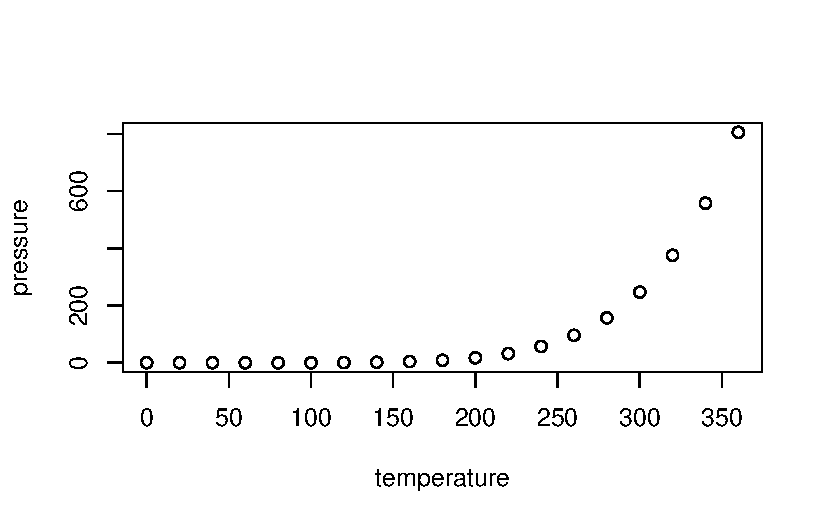
\includegraphics{content/rmarkdown_files/figure-pdf/fig-pressure-1.pdf}

}

\caption{\label{fig-pressure}Plot of pressure}

\end{figure}

Note that the \texttt{echo\ =\ FALSE} parameter was added to the code
chunk to prevent printing of the R code that generated the plot.

\hypertarget{including-tables}{%
\section{Including Tables}\label{including-tables}}

You can also embed tables and reference them with Table~\ref{tbl-iris}.

\begin{Shaded}
\begin{Highlighting}[]
\FunctionTok{library}\NormalTok{(knitr)}
\FunctionTok{kable}\NormalTok{(}\FunctionTok{head}\NormalTok{(iris))}
\end{Highlighting}
\end{Shaded}

\hypertarget{tbl-iris}{}
\begin{longtable}[]{@{}rrrrl@{}}
\caption{\label{tbl-iris}Iris Data}\tabularnewline
\toprule()
Sepal.Length & Sepal.Width & Petal.Length & Petal.Width & Species \\
\midrule()
\endfirsthead
\toprule()
Sepal.Length & Sepal.Width & Petal.Length & Petal.Width & Species \\
\midrule()
\endhead
5.1 & 3.5 & 1.4 & 0.2 & setosa \\
4.9 & 3.0 & 1.4 & 0.2 & setosa \\
4.7 & 3.2 & 1.3 & 0.2 & setosa \\
4.6 & 3.1 & 1.5 & 0.2 & setosa \\
5.0 & 3.6 & 1.4 & 0.2 & setosa \\
5.4 & 3.9 & 1.7 & 0.4 & setosa \\
\bottomrule()
\end{longtable}

\bookmarksetup{startatroot}

\hypertarget{rendering-with-code}{%
\chapter{Rendering with Code}\label{rendering-with-code}}

You can have code (R, Python or Julia) in your qmd file. You will need
to have these installed on your local computer, but presumably you do
already if you are adding code to your qmd files.

\begin{Shaded}
\begin{Highlighting}[]
\NormalTok{x }\OtherTok{\textless{}{-}} \FunctionTok{c}\NormalTok{(}\DecValTok{5}\NormalTok{, }\DecValTok{15}\NormalTok{, }\DecValTok{25}\NormalTok{, }\DecValTok{35}\NormalTok{, }\DecValTok{45}\NormalTok{, }\DecValTok{55}\NormalTok{)}
\NormalTok{y }\OtherTok{\textless{}{-}} \FunctionTok{c}\NormalTok{(}\DecValTok{5}\NormalTok{, }\DecValTok{20}\NormalTok{, }\DecValTok{14}\NormalTok{, }\DecValTok{32}\NormalTok{, }\DecValTok{22}\NormalTok{, }\DecValTok{38}\NormalTok{)}
\FunctionTok{lm}\NormalTok{(x }\SpecialCharTok{\textasciitilde{}}\NormalTok{ y)}
\end{Highlighting}
\end{Shaded}

\begin{verbatim}

Call:
lm(formula = x ~ y)

Coefficients:
(Intercept)            y  
      1.056        1.326  
\end{verbatim}

You will need to change the GitHub Action in \texttt{.github/workflows}
to install these and any needed packages in order for GitHub to be able
to render your webpage. The GitHub Action install R since I used that in
\texttt{code.qmd}. If you use Python or Julia instead, then you will
need to update the GitHub Action to install those.

If getting the GitHub Action to work is too much hassle (and that
definitely happens), you can alway render locally and publish to the
\texttt{gh-pages} branch. If you do this, make sure to delete or rename
the GitHub Action to something like

\begin{verbatim}
render-and-publish.old_yml
\end{verbatim}

so GitHub does not keep trying to run it. Nothing bad will happen if you
don't do this, but if you are not using the action (because it keeps
failing), then you don't need GitHub to run it.

\hypertarget{render-locally-and-publish-to-gh-pages-branch}{%
\section{Render locally and publish to gh-pages
branch}\label{render-locally-and-publish-to-gh-pages-branch}}

To render locally and push up to the \texttt{gh-pages} branch, open a
terminal window and then \texttt{cd} to the directory with the Quarto
project. Type this in the terminal:

\begin{verbatim}
quarto render gh-pages
\end{verbatim}

\bookmarksetup{startatroot}

\hypertarget{references-1}{%
\chapter{References}\label{references-1}}

Quarto has powerful references functionality. You can easily insert
citations from Zotero libraries that you maintain in the cloud (on
Zotero). This allows the whole team to update the library and you can
sync up to that library. Read about this on the Quarto documentation on
\href{https://quarto.org/docs/visual-editor/technical.html\#citations}{citations}.
Google youtube videos on this also to see it in action.

Add a \texttt{.bib} file in to your project or add a linked Zotero
library via RStudio in Visual mode with Tools \textgreater{} Project
Options\ldots{} \textgreater{} R Markdown \textgreater{} select custom
libraries from the Zotero dropdown.

The you can type \texttt{@} and you will see a dropdown of the
references in your libraries. You can then select the ones to add. If
you don't see the one you need, you can paste in the DOI and it will be
added to your references file (with all the info). The references will
be added to your references section of your book automatically.

See the \texttt{references.qmd} file for how to include the references.

\begin{itemize}
\item
  \texttt{@ansley1981} will produce Ansley \& Davis (1981)
\item
  \texttt{{[}@ansley1981{]}} will produce (Ansley \& Davis, 1981).
\end{itemize}

\bookmarksetup{startatroot}

\hypertarget{references-2}{%
\chapter*{References}\label{references-2}}
\addcontentsline{toc}{chapter}{References}

\markboth{References}{References}

\hypertarget{refs}{}
\begin{CSLReferences}{1}{0}
\leavevmode\vadjust pre{\hypertarget{ref-ansley1981}{}}%
Ansley, H. L. H., \& Davis, C. D. (1981). \emph{Migration and standing
stock of fishes associated with artificial and natural reefs on
georgia{'}s outer continental shelf} (p. 38).

\end{CSLReferences}


\backmatter

\end{document}
